\documentclass[sn-mathphys,Numbered]{sn-jnl}

\usepackage{xcolor}
\usepackage{graphicx}
\usepackage{amsthm}
\usepackage{amsmath}
\usepackage{algorithm}
\usepackage{algpseudocode}
%\usepackage[colorlinks=true, allcolors=blue]{hyperref}
\usepackage[numbers,sort&compress]{natbib}
\usepackage{soul}
\usepackage[percent]{overpic}
\usepackage[T1]{fontenc}
\usepackage[utf8]{inputenc}


\theoremstyle{definition}
\newtheorem{definition}{Definition}[section]

\begin{document}

\title[Direction-aware TDA]{Direction-aware topological descriptors for Young's modulus prediction in porous materials}

\author*[1,2]{Rafał Topolnicki}
\email{rafal.topolnicki@uwr.edu.pl}

\author[1]{Michał Bogdan}
\author[3]{Jakub Malinowski}
\author[1,4]{Bartosz Naskręcki}
\author[5]{Maciej Harańczyk}
\author[1]{Paweł Dłotko}

\affil[1]{Dioscuri Center in Topological Data Analysis, Institute of Mathematics, Polish Academy of Sciences, ul.
Sniadeckich 8, 00-656 Warsaw, Poland}
\affil[2]{Institute of Experimental Physics, University of Wrocław, pl. Maxa Borna 9, Wrocław 50-204, Poland}
\affil[3]{Faculty of Pure and Applied Mathematics, Wrocław University of Science and Technology, ul. Wybrzeże Wyspiańskiego 27, 50-370 Wrocław, Poland}
\affil[4]{Faculty of Mathematics and Computer Science, Adam Mickiewicz University, ul. Uniwersytetu Poznańskiego
4, 61-614 Poznań, Poland}
\affil[5]{IMDEA Materials Institute, C. Eric Kandel 2, Getafe, 28906 Madrid, Spain}

\abstract{
\textit{
Classical topological descriptors used in topological data analysis (TDA) are invariant under permutations of spatial axes and therefore cannot represent the loading direction, which is essential for modeling anisotropic mechanical response. Here, this limitation is addressed by introducing a \emph{direction-aware TDA framework} in which the compression axis is explicitly embedded into filtration functions used to compute both persistent homology and Euler characteristic profile descriptors. Across multiple porous-material datasets spanning a broad range of structural anisotropy, direction-aware descriptors yield higher predictive accuracy than their direction-agnostic counterparts, with performance gains that increase systematically with anisotropy. Notably, direction-aware descriptors remain competitive and often improve $R^2$ even for nominally isotropic ensembles, indicating sensitivity to mechanically relevant directional organization beyond bulk anisotropy measures. When used as inputs to gradient-boosted tree models, the proposed descriptors approach the accuracy of convolutional neural networks trained directly on voxelized structures while retaining a compact, transferable representation. The study considers multiple datasets spanning weak to strong anisotropy, enabling systematic validation of direction-aware topology across regimes. Overall, the results establish direction-aware TDA as a general route for linking porous structure to direction-dependent elastic properties and motivate its use in anisotropic materials modeling problems where a preferred direction naturally arises.}
}
\maketitle

\section{Introduction}
Porous materials consist of interconnected regions of solid matter and voids, which may be filled with a gas or liquid.  Porous and nanoporous metals, in particular, have found widespread applications in chemical catalysis, plasmonics, and spectroscopy~\cite{Koya2021}, as orthopedic implants~\cite{Guo2025,Matassi2013,Depboylu2024}, in energy storage technologies, and as the basis for strong, ultralight structural materials~\cite{Schaedler2016}. In many of these applications, the mechanical performance of porous metals—encompassing stiffness, strength, deformation behavior, and failure—plays a critical role in determining functionality, durability, and reliability.


Despite decades of research, establishing predictive relationships between porous structure and mechanical properties remains challenging. In particular, predicting the dependence of Young’s modulus on microstructural features such as porosity, pore morphology, and connectivity is nontrivial. Most existing approaches rely on scaling relationships between material density and tensile or compressive moduli, derived from empirical observations or simplified theoretical models.
The widely used and theoretically well-justified Gibson-Ashby model~\cite{Gibson1982} postulates a power-law relationship between material density $\rho$ and Young's modulus $E \propto \rho^n$. This foundational model predicts $E \propto \rho^2$ for open-cell porous materials and $E \propto \rho^3 $ for materials with closed pores~\cite{Gibson1982}. 
However, many types of materials violate the Gibson-Ashby model. In some open-celled nanoporous metal structures Young's modulus grows faster with density than the model's predictions suggest~\cite{Badwe2017}, while in others it grows slower~\cite{Zheng2014}. While this makes it clear that the porosity of a porous material itself does not determine its Young's modulus and geometrical and topological details of the solid material and pores also play key roles, no general functional relationship between Young's modulus and topology is known. 

Topological data analysis (TDA) offers a principled mathematical framework for quantifying such structural features across multiple length scales. By characterizing connectivity, loops, and cavities in a scale-dependent manner, TDA provides compact summaries of complex structures that are robust to noise and discretization. Tools such as persistent homology, persistence diagrams, Euler characteristic curves, and Euler characteristic profiles encode how topological features emerge and disappear as a structure is coarse-grained. Importantly, these descriptors can be efficiently computed for large datasets and subsequently vectorized for use in machine-learning pipelines~\cite{Krishnapriyan2021,Moon2019}.

A limited number of such TDA-involving attempts to predict the properties of porous materials have been reported. The existing results suggest TDA can be helpful in quantifying the heterogeneity of porous materials and predicting properties related to flow transport, permeability, fluid trapping and dissolution properties under reactive transport~\cite{Robins2016, Herring2019, Moon2019, Thompson2023, Lisitsa2020}, classifying  metal-organic frameworks based on their gas adsorption potential~\cite{Lee2017} and predicting the efficiency of the adsorption~\cite{Krishnapriyan2021, Chen2025, Wang2025, Lee2017}. A relationship has been found between persistent homology and elastic modulus in a sample of rock structures ~\cite{Jiang2018} and a similar study was conducted for wet compact powders~\cite{Ishihara2023}, however, both of these studies are affected by a very small sample sizes.

A key limitation of existing TDA approaches in this context is their inherent isotropy. Standard topological descriptors are invariant under rotations and reflections and therefore do not encode directional information or account for the breaking of symmetry with respect to the principal axes. This poses a fundamental obstacle for modeling anisotropic mechanical response in porous materials, where uniaxial Young’s modulus depends strongly on the loading direction and different axes may act as mechanically easy or hard directions. As a result, direction-agnostic topological summaries cannot distinguish between structurally identical but mechanically inequivalent orientations, making them unsuitable for predicting direction-dependent properties such as uniaxial stiffness or strength in anisotropic porous solids.

In this work, a direction-aware TDA framework is introduced by embedding the loading axis directly into filtration functions and systematically evaluating the resulting descriptors for uniaxial Young’s modulus prediction. To this end, we construct datasets spanning a wide range of structural anisotropy and demonstrate that directional TDA descriptors achieve substantially higher predictive performance than the non-directional descriptors commonly used in the literature. 
For strongly anisotropic structures, direction-aware descriptors provide large gains in both $R^2$ (coefficient of determination) and MAE (Mean Absolute Error), while for nominally isotropic datasets they remain uniformly competitive and typically improve $R^2$, indicating that direction-aware topology captures mechanically relevant organization even when macroscopic anisotropy is weak.
To verify that these findings are not specific to a particular structure class or generation mechanism, we further evaluate the approach on additional datasets encompassing diverse porous topologies and controlled anisotropy levels, recovering the same qualitative trends. Across all datasets, direction-aware persistent homology and multifiltration Euler characteristic profiles yield superior predictive performance, with the performance gap increasing systematically with structural anisotropy. When combined, directional PH and ECP descriptors achieve predictive accuracy approaching that of convolutional neural networks trained directly on voxelized structure data, while remaining orders of magnitude more compact and offering substantially greater interpretability.

This paper is organized as follows. Section~2 describes the datasets of porous structures used in this study, including the procedures for dataset generation and the numerical estimation of uniaxial Young’s modulus using FFT-based simulations. Section~3 introduces the construction of both directional and non-directional topological descriptors, detailing the formulation of force-direction-aware scalar and vector fields for persistent homology and Euler characteristic profiles. Section~4 presents and analyzes the results of the proposed direction-aware TDA-based predictive models and compares their performance with the non-directional counterparts and with convolutional neural networks trained directly on voxelized structures, demonstrating the advantages of incorporating directional topology. Section~5 summarizes the main findings and discusses their implications.

\section{Dataset}

\subsection{Random Trigonometric Phase}

The porous two-phase structures used in this study were generated using a
\emph{random trigonometric phase} (RTP) approach, in which a continuous,
statistically homogeneous random field is constructed as a superposition of
trigonometric modes with random phases and wavevectors.


We consider a cubic domain discretized on a regular
$N \times N \times N$ grid with $N=80$ and periodic boundary conditions.
The spatial coordinates are normalized to the unit cube,
$\mathbf{x} \in [0,1)^3$, and periodicity is enforced implicitly by the
trigonometric basis.
The RTP scalar field $S(\mathbf{x})$ is defined as
\begin{equation}
\label{eqn:rtp_S}
S(\mathbf{x}) =
\sqrt{\frac{2}{K}}
\sum_{k=1}^{K}
\cos\!\left( 2\pi\,\mathbf{q}_k \cdot \mathbf{x} + \phi_k \right),
\end{equation}
where $K$ is the number of trigonometric modes,
$\phi_k \sim \mathcal{U}(0,2\pi)$ are independent random phase shifts, and the
wavevectors $\mathbf{q}_k$ are sampled from a bounded integer lattice $\mathbf{q}_k = (n_x, n_y, n_z), n_\alpha \in [-n_\text{max}, n_\text{max}].$
Because each cosine mode is periodic on the unit torus, the field $S$ and all
derived microstructures satisfy periodic boundary conditions by construction.

The continuous field $S(\mathbf{x})$ is converted into a binary porous medium
by thresholding.
The material indicator function $X(\mathbf{x}) \in \{0,1\}$ is defined as
\[
X(\mathbf{x}) =
\begin{cases}
1, & S(\mathbf{x}) > \tau, \\
0, & \text{otherwise},
\end{cases}
\]
where $X=1$ denotes solid material and $X=0$ denotes void.
For each realization, the threshold $\tau$ is determined numerically such that
the resulting porosity $\phi$ matches a prescribed target value, selected
prior to generation.
To ensure physically meaningful structures, each realization is subjected to a
connectivity and percolation analysis under periodic boundary conditions:
all material voxels must form a single connected component and the solid phase
must percolate across the domain in all three Cartesian directions, otherwise the structure is not included in the dataset.
In this study, we used $K$ values sampled uniformly from the interval $[10, 30]$, fixed $n_{\text{max}} = 12$, and selected the target porosity uniformly from the interval $[0.2, 0.8]$.


In the isotropic case, the statistical properties of $S$ are invariant under
rotations, as the spectral content is identical on average along all spatial
directions.
Directional anisotropy is introduced explicitly in Fourier space by scaling
the components of the wavevectors prior to evaluating Eq.~\eqref{eqn:rtp_S}.
Specifically, integer wavevectors $\mathbf{q}_k^{(0)}$ are first sampled
uniformly from the bounded lattice, and the final wavevectors are defined as
\begin{equation*}
\mathbf{q}_k = \mathrm{diag}(s_x, s_y, s_z)\,\mathbf{q}_k^{(0)},
\end{equation*}
where $(s_x, s_y, s_z)$ are prescribed anisotropy scaling factors.
This construction directly controls the characteristic correlation lengths of
the random field: larger values of $s_\alpha$ correspond to higher spatial
frequencies and thus shorter correlation lengths along direction $\alpha$,
whereas smaller values of $s_\alpha$ lead to longer-range correlations.

In this work, we set $s_x = s_y = 1$ and $s_z = 0.2$, resulting in structures
with significantly extended correlation length along the $z$ axis and a
pronounced directional anisotropy.

\begin{figure}
    \centering
    \begin{overpic}[width=0.3\textwidth]{render_rtp_420.png}
        \put(5,85){\large a}
    \end{overpic}
    \begin{overpic}[width=0.3\textwidth]{render_rtp_121.png}
        \put(5,85){\large b}
    \end{overpic}
    \begin{overpic}[width=0.3\textwidth]{render_rtp_349.png}
        \put(5,85){\large c}
    \end{overpic}
    \caption{
    Three exemplary RTP structures illustrating increasing structural and mechanical anisotropy. The directional Young’s moduli $E=(E_x,E_y,E_z)$ are: (a) $(10.3, 11.3, 31.4)\,\mathrm{GPa}$, (b) $(5.2, 10.0, 33.1)\,\mathrm{GPa}$, and (c) $(19.8, 17.5, 51.2)\,\mathrm{GPa}$. The corresponding porosities are $0.60$, $0.54$, and $0.68$, while the spectral anisotropy components $k=(k_x,k_y,k_z)$ are $(0.63, 0.69, 0.27)$, $(0.98, 0.89, 0.25)$, and $(1.00, 1.20, 0.19)$, respectively. The progressive reduction of $k_z$ relative to $k_x$ and $k_y$ reflects increasing elongation along the $z$ direction, consistent with the growing contrast between in-plane and out-of-plane Young’s moduli.
        }
    \label{fig:rtp}
\end{figure}

A total of 500 distinct RTP microstructures were generated. For each structure, uniaxial compression tests were performed independently along the three Cartesian directions, and the corresponding directional Young’s moduli were computed using an FFT-based spectral homogenization method implemented in \texttt{FFTMAD} (see Section~\ref{sec:fftmad} for details of the numerical procedure). Figure~\ref{fig:rtp} presents three exemplary RTP structures spanning increasing levels of structural anisotropy, together with their corresponding directional Young’s moduli, porosities, and spectral anisotropy measures, illustrating correlation between directional morphology and mechanical response.

\subsection{Dataset of topologically diverse structures}
\label{sec:td_structures}
A dataset of 2375 topologically diverse (TD) 
periodic porous structures was generated to assess the
generality of the proposed topological descriptors beyond RTP-based structures.
All structures occupy a normalized $1\times1\times1$ cubic domain, voxelized on a
regular $80\times80\times80$ grid, and satisfy periodic boundary conditions in all three spatial
directions.
Importantly, the dataset was constructed to be \emph{statistically isotropic}:
no preferred spatial direction is imposed by the generation procedures, and the
resulting ensembles exhibit no systematic directional bias in their geometric
or mechanical properties.
Within this constraint, the dataset spans a broad range of pore morphologies and
topologies.
The dataset comprises five approximately equally sized subsets, each
corresponding to a distinct family of porous structures generated by a
different stochastic algorithm.
Within each family, randomness ensures substantial variability in geometric
features and effective elastic properties while preserving statistical
isotropy. Additional details on the generating algorithms are available in the SI, while the full dataset, together with the corresponding unidirectional Young’s moduli, is available in the dedicated repository associated with this paper -- see section Code and Data Availability for more information.
The five structure families are referred to as Voronoi, Zeolitic, Diamond-like,
Cubic-strut, and Spline-based structures.
Representative examples and generation schematics are shown in
Figure~\ref{fig:various_aniso}.
Below we briefly summarize the defining characteristics of each family.

\paragraph{Voronoi-based structures} were generated from three-dimensional Voronoi
tessellations of randomly distributed seed points within the unit cell.
Between three and twelve points were sampled uniformly per realization, and the
edges of the resulting tessellation were used as the structural skeleton.
These edges were voxelized and thickened to form struts with square cross
sections of randomly varying thickness (see Figure~S1 in the Supplementary Information).

\paragraph{Zeolitic-inspired structures} were derived from predicted zeolite frameworks reported in
the database of Deem and co-workers~\cite{C0CP02255A,deem2023pcod}.
A subset of structures with orthogonal unit cells was selected and rescaled to
the normalized cubic domain.
Although individual realizations may exhibit complex internal connectivity, the
ensemble does not privilege any spatial direction and is therefore
statistically isotropic.

\paragraph{Diamond-like structures} were generated by perturbing the atomic positions of an
ideal diamond lattice within the unit cell.
Random displacements drawn from isotropic normal distributions were applied
uniformly to all lattice sites, with the displacement magnitude varied across
realizations.
Edges corresponding to nearest-neighbor bonds were then thickened to form struts
with randomly selected square cross sections, producing networks that remain
statistically isotropic at the ensemble level.

\paragraph{Cubic-strut structures} were generated using the same procedure as for the
diamond-like structures, but starting from a simple cubic lattice rather than a
diamond lattice.
Random perturbations of the lattice sites and variations in strut thickness
introduce geometric disorder while preserving the absence of any preferred
orientation in the ensemble.

\paragraph{Spline-based structures} were constructed by thresholding smooth, periodic scalar
fields defined via trivariate tensor-product B-splines.
Random spline coefficients were drawn independently, and periodicity was
enforced at the level of the spline basis.
Because the underlying scalar fields are generated without directional
preference, the resulting binary porous structures form a statistically
isotropic ensemble with smooth pore morphologies and controlled volume
fractions.

\subsection{Dataset of anisotropic transformed topologically diverse structures}
\begin{figure}
    \centering
    \begin{overpic}[width=0.18\textwidth]{render_splines.png}
        \put(5,85){\large a}
    \end{overpic}
    \begin{overpic}[width=0.18\textwidth]{render_diamond.png}
        \put(5,85){\large b}
    \end{overpic}
    \begin{overpic}[width=0.18\textwidth]{render_cubic.png}
        \put(5,85){\large c}
    \end{overpic}
    \begin{overpic}[width=0.18\textwidth]{render_zeolites.png}
        \put(5,85){\large d}
    \end{overpic}
    \begin{overpic}[width=0.18\textwidth]{render_voronoi.png}
        \put(5,85){\large e}
    \end{overpic}

    \caption{Examples of the five structure types used in the ATTD dataset: a: splines, b: diamond, c: cubic, d: zeolite, e: Voronoi-based structures.}
    \label{fig:various_aniso}
\end{figure}
For the TD dataset, there is no natural or
straightforward way to introduce anisotropy at the level of structure
generation.
To overcome this limitation and to enable a systematic study of anisotropic
effects, a simple geometric elongation procedure was applied to the existing
binary structures, yielding an additional dataset denoted Anisotropic Transformed Topologically Diverse (ATTD).

Each original isotropic structure, represented on an $80\times80\times80$
voxel grid, was first downsampled to a $40\times40\times40$ grid, forming a
coarse-grained structural segment.
This segment was then elongated along the $z$ direction to obtain a
$40\times40\times80$ volume.
Finally, the elongated segment was replicated four times in the transverse
directions to reconstruct an $80\times80\times80$ periodic grid.

This transformation preserves the local topology of the original structures
while introducing a distinguished spatial direction through geometric
elongation.
As a result, isotropy is systematically broken and a moderate, controllable
structural anisotropy is introduced, with the $z$ axis becoming preferentially
aligned.
The resulting dataset provides a complementary benchmark bridging the gap
between statistically isotropic diverse structures and the strongly anisotropic
RTP-based datasets.

\subsection{Anisotropy Measures}

Structural anisotropy was quantified directly on the binary voxelized
microstructures~\cite{PhysRevE.76.031110}. Two complementary measures were employed, capturing
anisotropy in real space and in Fourier space, respectively.

Directional correlation lengths were estimated from the two-point
autocorrelation function of the mean-centered indicator field
$Y(\mathbf{x}) = X(\mathbf{x}) - \langle X \rangle$.
For each Cartesian direction, one-dimensional periodic autocorrelation functions
were computed along all lines parallel to that axis using FFT-based convolution
and subsequently averaged over transverse coordinates.
The resulting directional autocorrelation functions $C_x(\ell)$, $C_y(\ell)$,
and $C_z(\ell)$ were normalized such that $C_\alpha(0)=1$.
We define directional correlation lengths $L_\alpha = \sum_{\ell \ge 0} C_\alpha(\ell)$ 
where the sum is restricted to non-negative lags up to the first zero crossing of
$C_\alpha(\ell)$ as a characteristic anisotropy length. 
Structure anisotropy is additionally characterized in Fourier space using the power
spectrum. The discrete Fourier transform of the mean-centered indicator field was computed
and the directional second moments of the power spectrum, $\langle k_\alpha^2\rangle$, were evaluated by weighting each squared wavevector component by the normalized spectral power.
To reduce sensitivity to interface-induced high-frequency noise inherent to
binary data, the spectral moments were computed after removal of the zero
frequency mode. 
Together, these real-space and spectral measures provide quantification 
of anisotropy in all porous materials considered here. 


\subsection{Estimation of the Young's modulus}
\label{sec:fftmad}

Effective Young’s moduli of the porous microstructures were computed in silico
using an FFT-based homogenization approach implemented in the Python package
\texttt{FFTMAD}~\cite{Lucarini2019}.
For each structure, uniaxial compressive loading was applied along the selected
principal directions, and the effective Young’s modulus was extracted from the
linear macroscopic stress--strain response.

For the RTP datasets, the solid phase was modeled as an isotropic linear elastic
material with Young’s modulus $E_{\mathrm{bulk}}=\text{81.5}\,\mathrm{GPa}$ and
Poisson’s ratio $\nu_{\mathrm{bulk}}=\text{0.39}$, chosen to be representative of the
Au$_{0.30}$Ag$_{0.70}$ alloy -- a material frequently used in nanoporous research~\cite{ShanShi, ZANDERSONS2021116979, BEETS2021116445}. 
The elastic properties of the structures in the TD and ATTD were set to $E_{\mathrm{bulk}}=\text{70.0}\,\mathrm{GPa}$ and $\nu_{\mathrm{bulk}}=\text{0.33}$ and correspond to aluminium.
All simulations were performed in the small-strain regime, and on the voxelized
structures. 

\section{Background and methods}
\subsection{Computing topological descriptors on the structures}
\begin{figure}
    \centering
    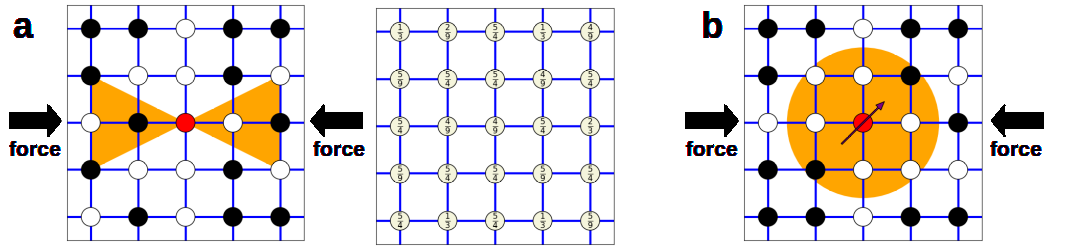
\includegraphics[width=\textwidth]{TDA_directional_horizontal_new.png}
    \caption{Diagrams \textbf{a} and \textbf{b} illustrate the calculation of filtration based on cones and principal components, respectively. The actual filtrations were calculated for three-dimensional grids, but for clarity, the examples are two-dimensional. Black and red circles represent non-empty fragments of material, while white circles represent empty spaces. In both cases, the filtration value is calculated for the central element marked in red.
    In the first image of diagram \textbf{a}, there are 5 non-empty and 4 empty elements in the constructed cones (orange triangles), so the filtration for the middle point is equal to $4/9$.
    By applying this procedure to other grid points, we obtain the grid of numbers presented in the second image in diagram \textbf{a}.
    In diagram \textbf{b}, if we limit ourselves only to elements contained in a certain neighborhood (orange circle), all non-empty elements will lie along one direction (marked with a purple arrow). This direction is the basis for calculating the multifiltration value.}
    \label{fig:TDA_directional}
\end{figure}

\subsubsection{Topological data analysis}

Topological data analysis (TDA) leverages the tools of topology and algebra to extract relevant information from datasets. The fundamental principle of this methodology is that "Data has shape and shape has meaning"~\cite{Dlotko2024}. The reader is referred to~\cite{Dlotko2024, Gurnari2025} for a comprehensive overview of the basic concepts. Here, we present a brief outline of the TDA methods we will use. 



To represent the topology of the structures, we used 3-dimensional cubical complexes, which consist of cubes of various dimensions. TDA enables the analysis of data structures at multiple resolutions, which are defined using a function called filtration~\cite{Dlotko2024, Gurnari2025}. The initial values of this function were computed for 0-dimensional cubes (vertices) and then propagated to higher-dimensional cells in a standard manner, known as V-construction~\cite{Robins2011}.

The filtrations chosen in previous applications of TDA to porous materials are based on the distance transform and therefore do not account for directionality~\cite{Robins2016, Herring2019, Moon2019, Thompson2023, Lisitsa2020, Lee2017, Krishnapriyan2021, Chen2025, Wang2025, Jiang2018, Ishihara2023}. However, directionality is a critical factor for anisotropic materials whose Young's modulus depends on the direction of compression. To address this, we encoded the compression direction information into the filtration functions, thereby making our descriptors direction-aware. The details of these functions are described in the next section.

\subsubsection{Cone-based filtration}

The first directional filtration we consider is based on porosity inside cones. For each element of the input grid two cones starting at this point and having rotational axis parallel to direction of compressions are constructed. The cones are positioned in opposite directions. In the case of extreme grid elements, the cones may extend beyond the boundaries of the defined material. Therefore, for calculation purposes, we assume that the material is periodic. Porosity inside the cones is filtration value assigned to vertex corresponding to selected element of the grid. If the grid element represents an empty space, the corresponding filtration value is set to 1.25. The value 1.25 is selected arbitrary so that all the grid points outside material enters the filtration after all the grid elements belonging to material (that have filtration values between 0 and 1). This is to make a clear distinction between empty and non-empty spaces in the structure. The method is presented graphically in the Figure~\ref{fig:TDA_directional}. The formal definition of the described filtration is as follows.

\begin{definition}
A double cone with height $h$ and radius $r$ attached at point $e=(i_0, j_0, k_0)$ is defined as the following set of indices
\[ \mathrm{Cone}(e, r, h) = \left\{ (i, j, k) \in \mathcal{N}: |k - k_0| < h \land \sqrt{|i -i_0|^2 + |j -j_0|^2} \leq \frac{|k-k_0|r}{h}  \right\}  \]
\end{definition}

\begin{definition}
Let $G$ be a three-dimensional lattice (grid) of size $n \times n \times n$. The cone-based filtration associated with the vertex corresponding to the grid element $g_e$ is given by the expression
    \[F_{cone}(e; r,h) =1 - \frac{1}{|\mathrm{Cone}(e, r, h)|} {\sum_{(i,j,k) \in {\mathrm{Cone}}(e, r, h)}{g_{i'j'k'}}}, \]
    where $i' = i \mod n$, $ j' = j \mod n$, $ k' = k \mod n$ and $|\mathrm{Cone}(e, r, h)|$ is the number of voxels within the cone.
\end{definition}

Cone-based filtration distinguishes the direction of compression ($z$-axis here) and is invariant under rotation around an axis parallel to that direction. This method takes two parameters, the cone's height and radius of its base.

\subsubsection{Filtration's extension based on principal component}
In the next step, we extended our initial filtration method to include information about the local material direction within specific regions. The local material direction for each material was represented by two parameters, which we determined through the following procedure.

For a selected grid element e, we treated all non-zero grid elements within a centered sphere of a radius $r$ as a 3D point cloud. We then calculated the first principal component  of this cloud to define its primary directional axis. The resulting normalized vector was used to extract two components: one corresponding to the compression direction ($v_z$) and a second, independent component ($v_y$).

This process results in a 2-parameter filtration value, specifically $(1-|v_z|,1-|v_y|) $. This filtration is motivated by the principle that a material's ability to transfer stress is maximized when its orientation aligns with the imposed compression direction. The method requires a single hyperparameter: the radius of the point's neighborhood. A recap of this method is shown in the Figure {\ref{fig:TDA_directional}}

The hyperparameters used in the filtration procedures were fixed across all experiments. For the cone-based filtration, the cone height was set to $h_{\mathrm{cone}} = 6$ and the cone base radius to $r_{\mathrm{cone}} = 3$. The same geometric parameters were employed for both the single-parameter filtration used in persistent homology and the multifiltration used in Euler characteristic profile calculations. In the principal-component-based multifiltration, the neighborhood radius was set to $r_{\mathrm{PC1}} = 4$, defining the spherical region used to estimate the local material orientation.



\begin{algorithm}
\caption{An algorithm of computing principal component-based multifiltration}\label{alg:cap}
\textbf{Input} \\
  \hspace*{\algorithmicindent}  $G$ - binary grid representing material \\
  \hspace*{\algorithmicindent}  $(i, j, k)$ - coordinates of selected element \\
  \hspace*{\algorithmicindent}  $r$ - neighborhood's radius
\begin{algorithmic}
\Procedure{PcFiltration}{$G,(i,j,k),r$}
\If{$G[i,j,k] = 0$}
    \State \Return (1.25, 1.25)
\Else
    \State $neighborhood \gets \mathrm{get\_neighborhood(G, (i,j,k), r)}$
    \State $v \gets \mathrm{calculate\_first\_principal\_component}(neighborhood)$
    \State $v \gets v / |v|$ \Comment{Normalization of 1st principal component}
    \State \Return $(1 - |v[2]|, 1 - |v[1]|)$
\EndIf
\EndProcedure
\end{algorithmic}
\end{algorithm}


\subsubsection{Direction-aware topological descriptors}

The filtrations described above were applied to study the structures at various resolutions. Next, we generated their topological summaries using persistent homology (for cone-based filtration) and Euler characteristic profiles (ECP) (for multifiltration). Persistent Homology (PH) is a fundamental tool in TDA. It offers the advantage of simultaneously capturing structural features, such as connected components, rings, and voids, at various scales. While ECP offers a less detailed topological description, it is computationally very efficient and allows for the use of multiparameter filtrations.

In the case of Persistent Homology calculations, the assumption of periodicity of the material in the  compression direction was used. Euler characteristic profiles were calculated without assuming periodicity in any direction. 


Since most machine learning models require vector-formatted inputs, persistence diagrams were converted into persistence images~\cite{JMLR:v18:16-337}. Each diagram was mapped to a $10 \times 10$ image with birth and persistence ranges both set to $(0, 1.25)$. Persistence diagrams in dimensions 0, 1, and 2 were vectorized separately and subsequently concatenated into a single descriptor. Euler characteristic profiles were vectorized independently by sampling the multifiltration values on a $7 \times 7 \times 7$ grid.

\subsection{Estimation using boosting algorithm and neural networks}

Vectorized topological descriptors were used to train machine learning models aimed at predicting the elastic properties of the corresponding porous structures. Predictive models based on topological descriptors were trained using the CatBoost algorithm, a gradient-boosted decision tree method designed to provide strong performance and robustness on structured tabular data~\cite{Prokhorenkova2019}. As a baseline, we employed a convolutional neural network with the DenseNet-121 architecture, trained directly on voxelized representations of the structures. This architecture has previously been shown to achieve state-of-the-art performance for predicting mechanical properties of RTP-type porous structures~\cite{praca_z_madrytem}.

Model training was performed using $k$-fold cross-validation with $k = 8$. The entire dataset was divided into eight folds. For the first model, folds 1–6 were used for training, the 7th fold served as a validation set to detect overfitting and determine when to stop training, and the 8th fold was used as the test set. All metrics reported in this paper were computed exclusively on the test sets. The second model was trained on folds 2–7, validated on fold 8, and tested on fold 1, and so on. Thus, for each algorithm, a total of eight models were trained, and the overall performance was obtained by averaging the metrics across all test sets. Using cross-validation increases the robustness of the results to random data splits. Moreover, it ensures that each data point is used exactly once as a test instance, allowing the reported metrics to represent the entire dataset.

To prevent data leakage, all $k$-fold cross-validation splits were performed at the structure level (stratification). When multiple Young’s modulus values were obtained from the same structure under different loading directions, these samples were assigned jointly to the training, validation, or test set within each fold. This ensured that mechanical responses of a given structure were never split across different subsets, providing a strict and physically meaningful evaluation of model generalization.


\section{Results and Discussion}

Table~\ref{tab:metrics} summarizes the predictive performance of the evaluated descriptor configurations across all considered datasets. In addition to regression metrics, the table reports two scalar measures characterizing structural anisotropy: the spectral measure $k$ and the integral correlation-length-based measure $L$, both computed directly from the binary microstructures.

For each dataset, the reported quantities are the standard deviations $\sigma(k)$ and $\sigma(L)$. These were computed from the directional values $k_\alpha$ and $L_\alpha$ corresponding to the same loading axes used to evaluate Young’s modulus in a given dataset. For example, for the RTPxy dataset, $\sigma(k)$ is calculated from the collection of $k_x$ and $k_y$ values across all structures, and $\sigma(L)$ analogously from $L_x$ and $L_y$. In this way, $\sigma(k)$ and $\sigma(L)$ quantify the spread of anisotropic characteristics within each dataset: larger values indicate greater variability in directional morphology, while smaller values correspond to more structurally homogeneous ensembles.


\begin{figure}
    \centering
    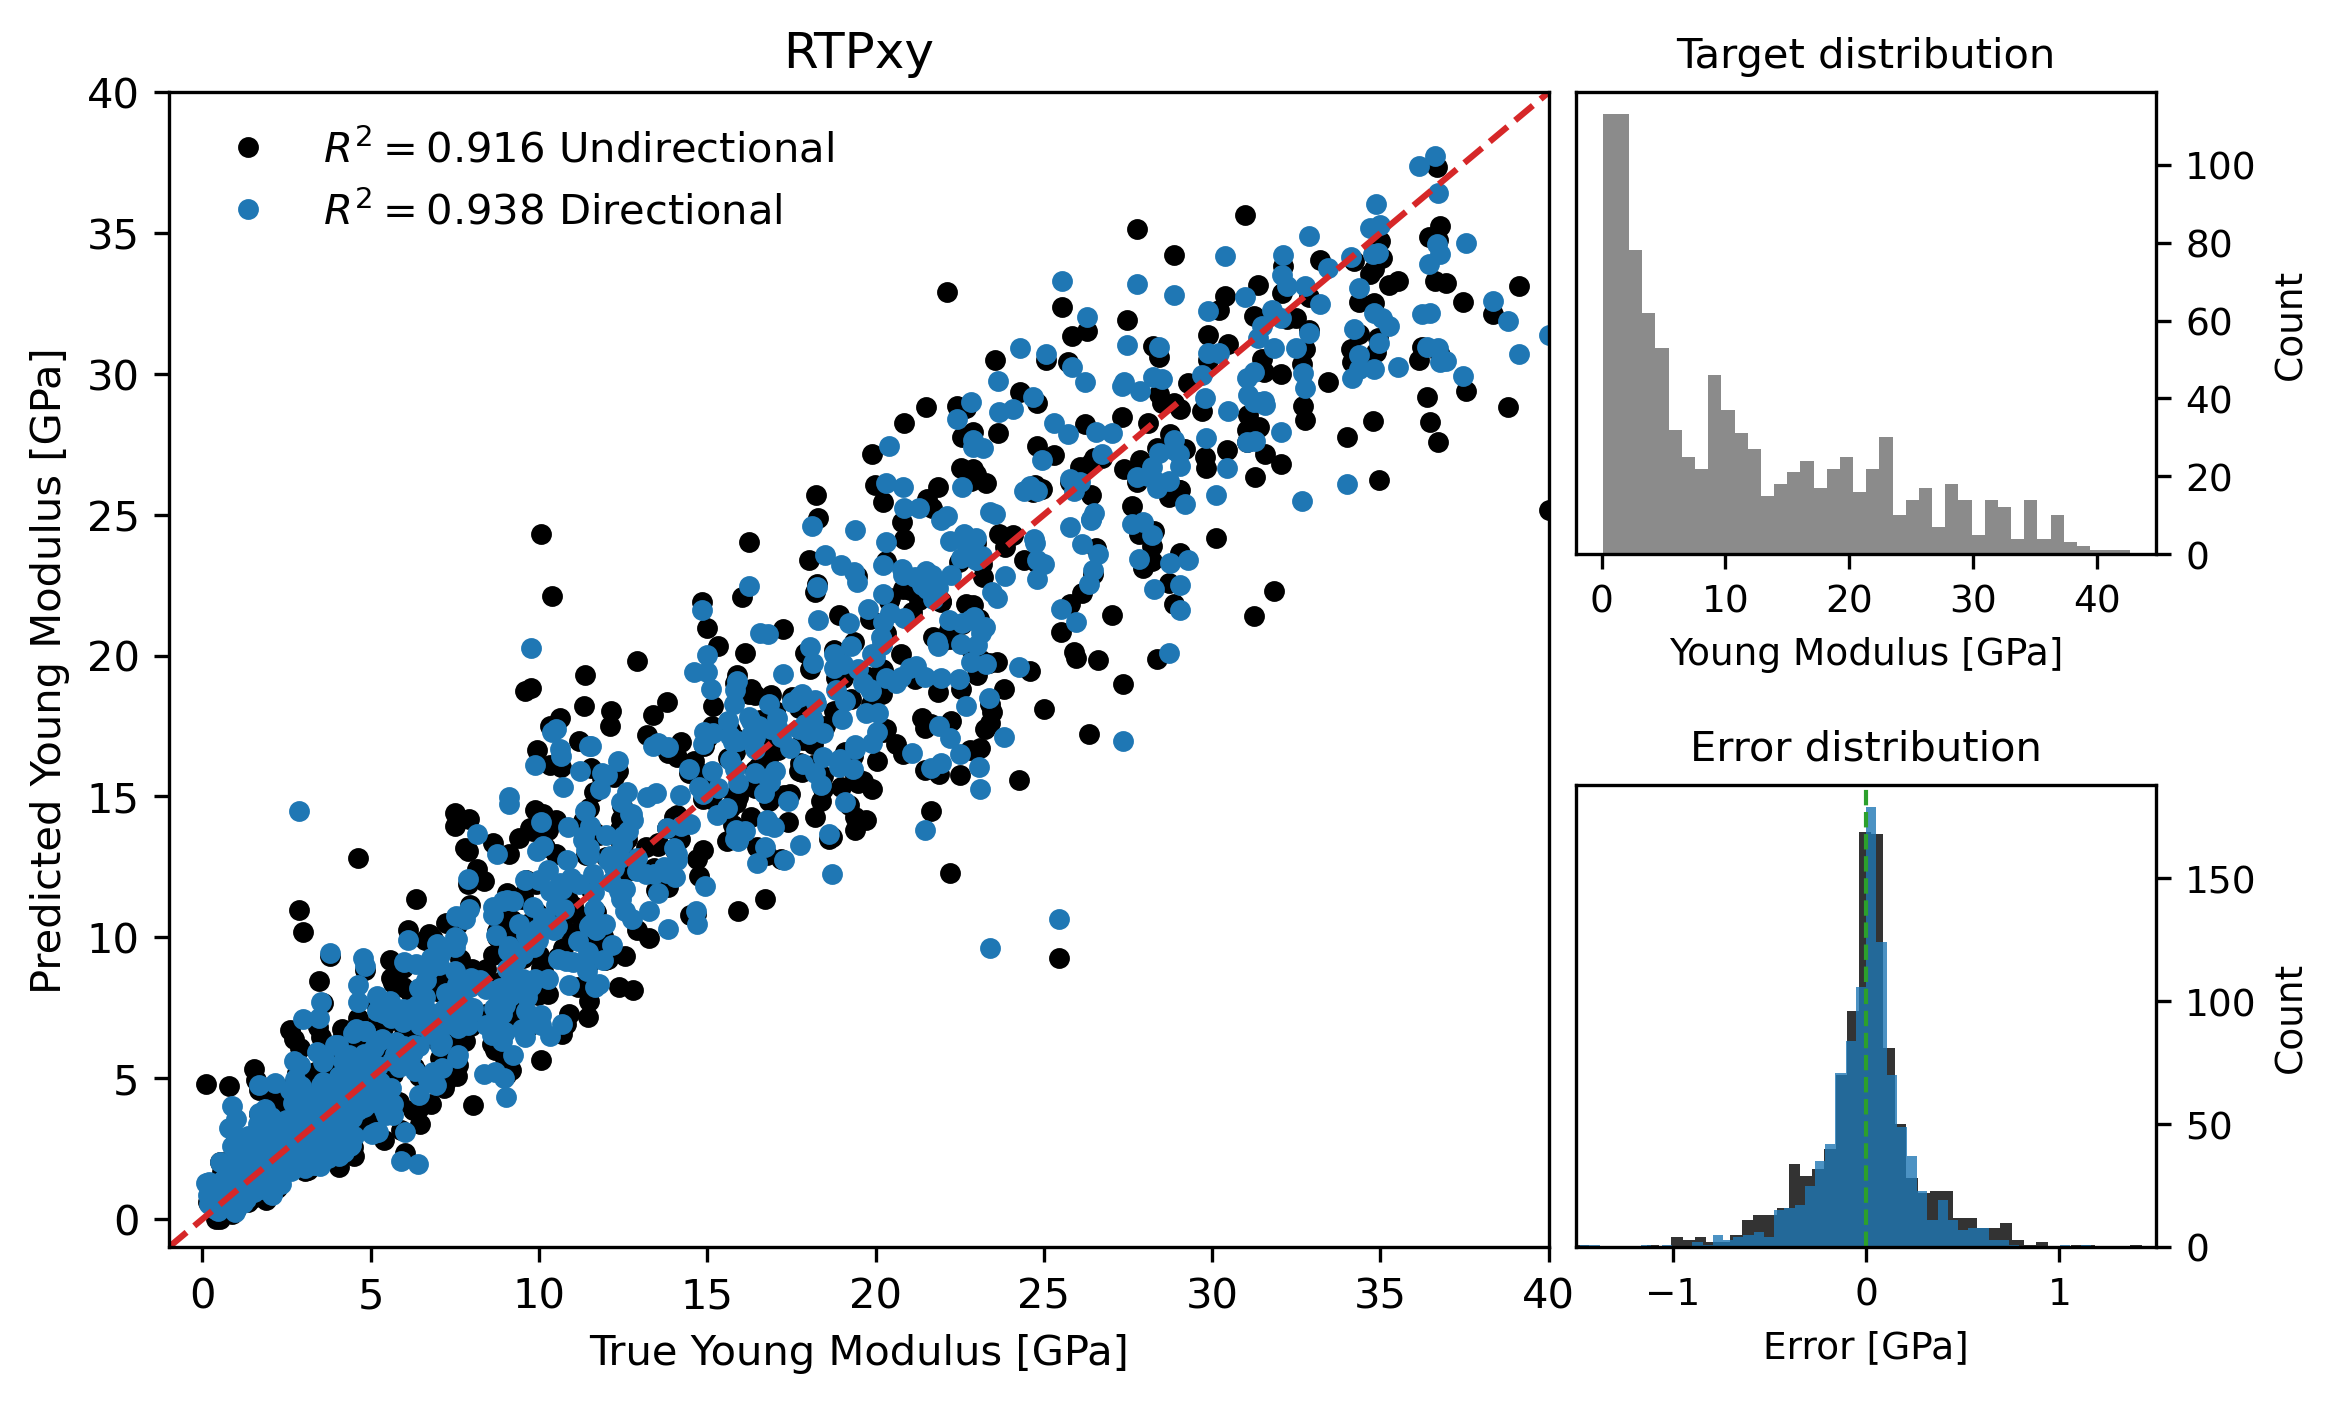
\includegraphics[width=0.495\linewidth]{scatter_rtp_xy.png}
    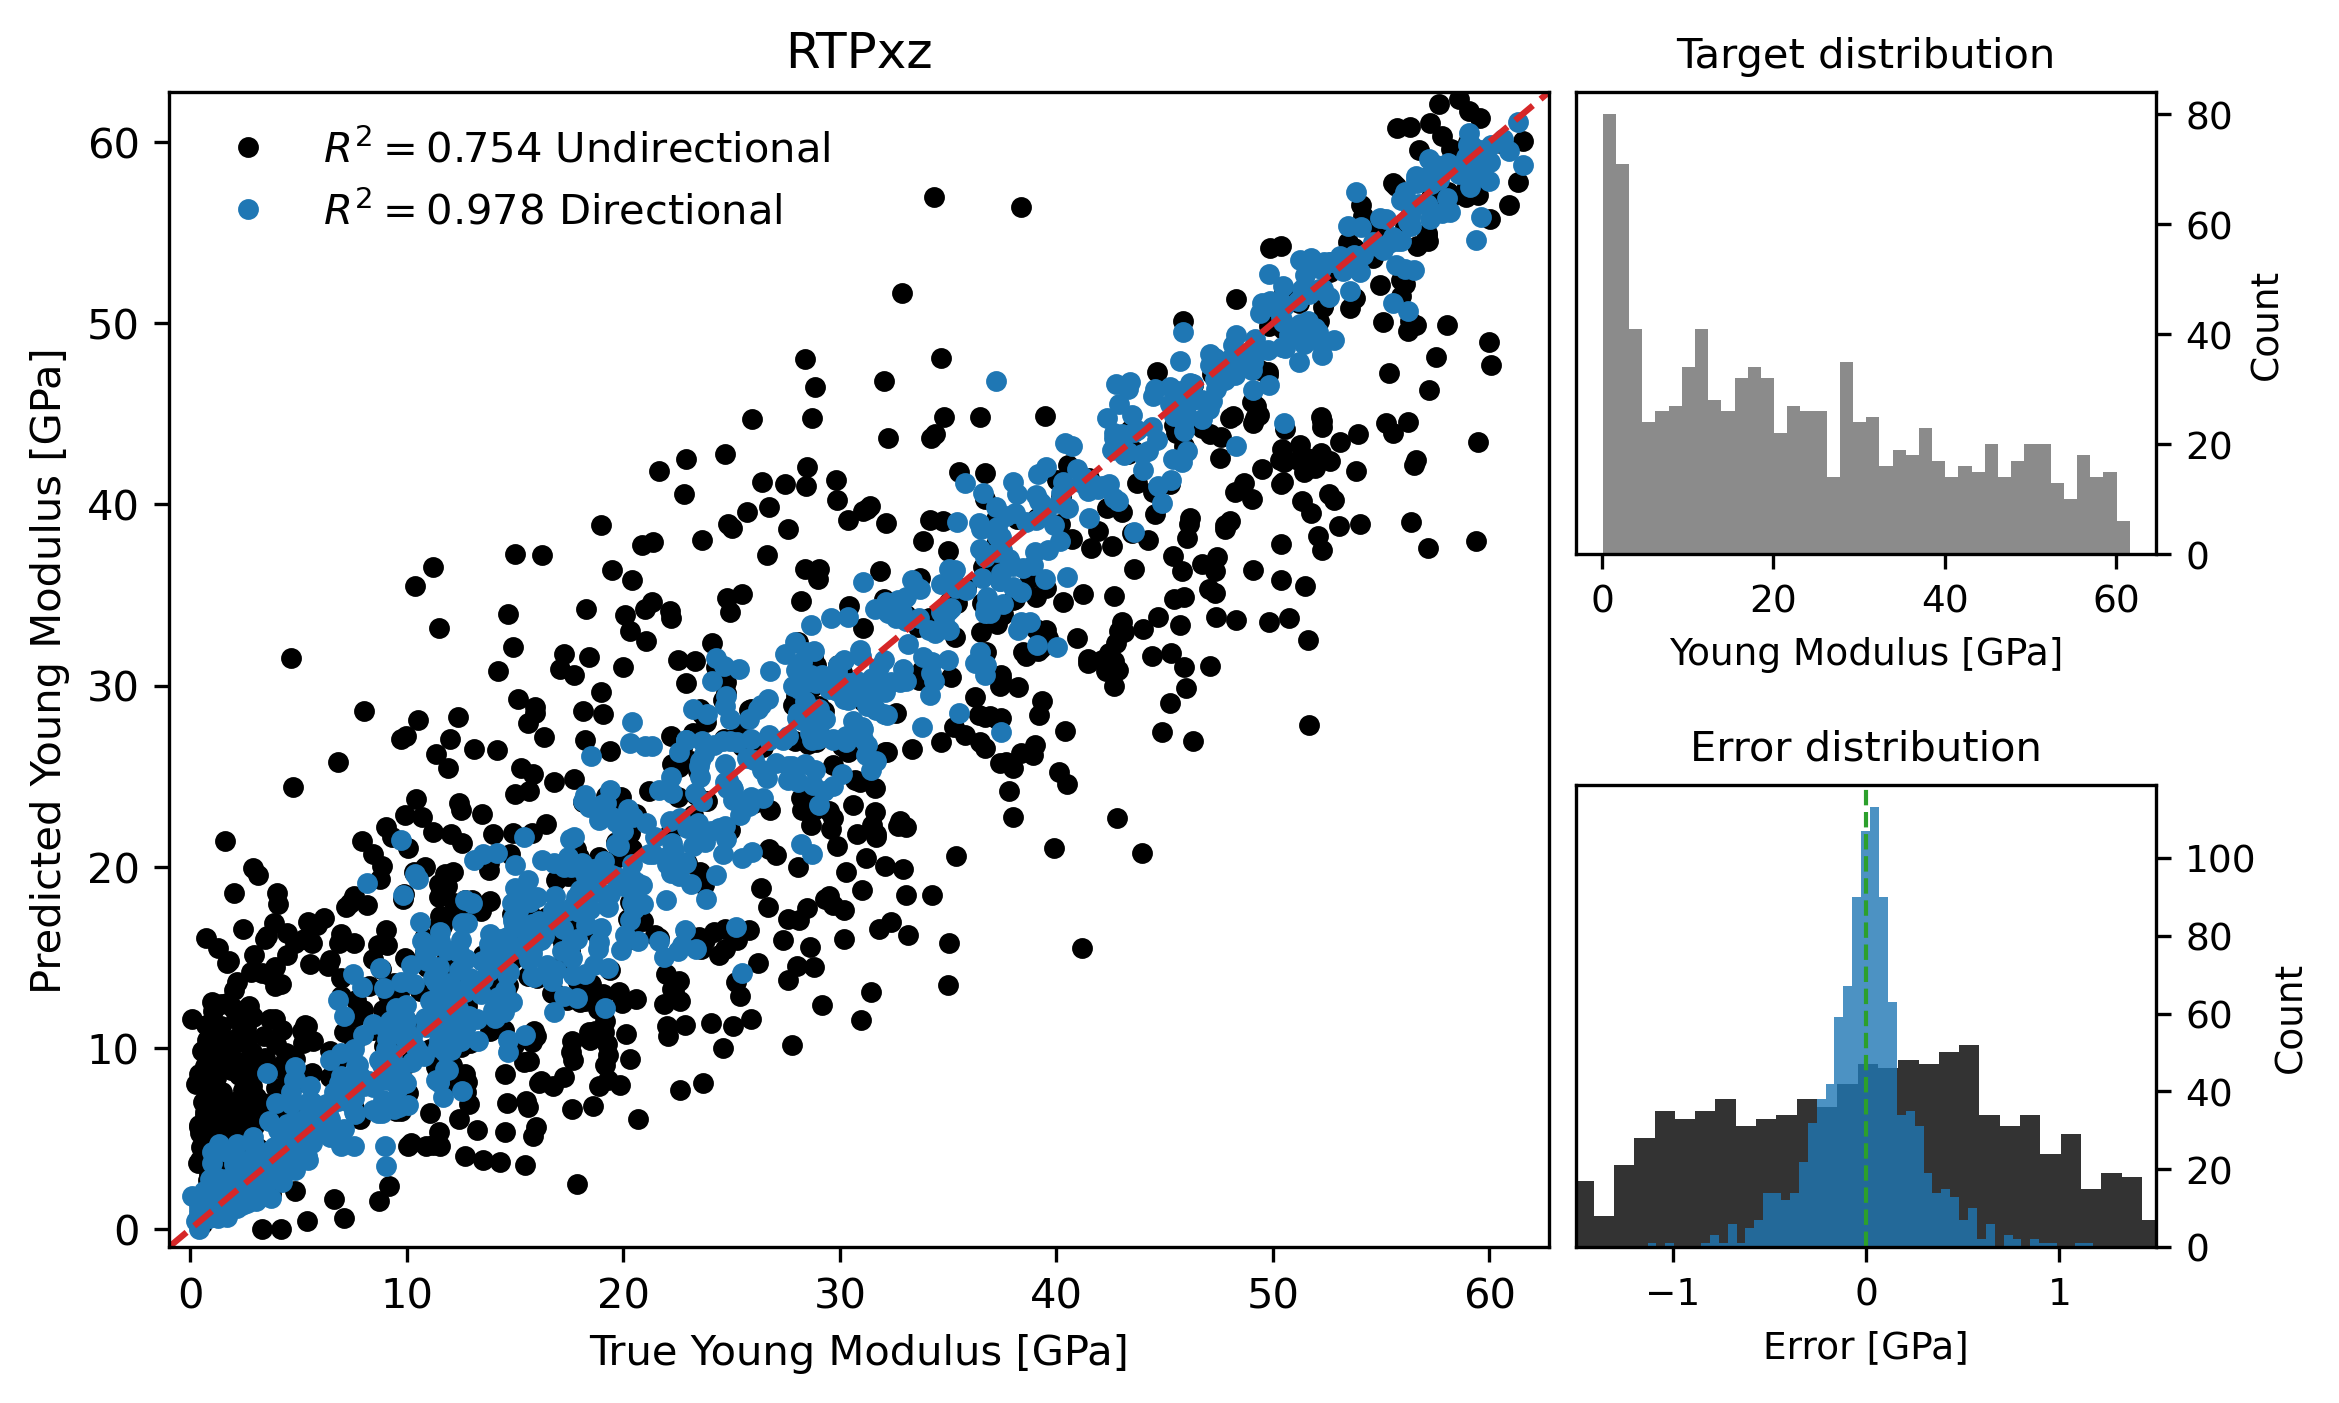
\includegraphics[width=0.495\linewidth]{scatter_rtp_xz.png}
    \caption{Predicted versus FFTMAD-computed Young’s modulus for the RTPxy (left panel) and RTPxz (right panel) datasets. In both cases, predictions were obtained using a CatBoost regression model trained on combined PH+ECP topological descriptors. The dashed line indicates perfect agreement between predicted and computed values. Black markers correspond to predictions based on non-directional descriptors, while blue markers denote predictions obtained using directional descriptors. Each panel includes two accompanying histograms: the upper histogram shows the distribution of Young’s modulus values in the dataset, and the lower histogram compares the distributions of prediction errors for non-directional and directional models.
    }
    \label{fig:scatter_rtp}
\end{figure}

Figure~\ref{fig:scatter_rtp} shows predicted versus FFTMAD-computed Young’s modulus for the RTPxy (left) and RTPxz (right) datasets. Insets display the distributions of Young’s modulus values (top) and prediction errors (bottom). For the weakly anisotropic RTPxy dataset, both directional and non-directional descriptors yield predictions tightly clustered around perfect agreement with narrow, symmetric error distributions. In contrast, for the strongly anisotropic RTPxz dataset, directional descriptors maintain high accuracy, while non-directional descriptors exhibit substantial deviations and broadened error distributions, highlighting the importance of directional topology under strong anisotropy.

The RTP datasets provide a controlled setting for assessing the influence of
structural anisotropy on predictive performance.
We first consider the RTPxy dataset, which consists of RTP microstructures for which Young’s modulus was evaluated exclusively
along the $x$ and $y$ directions.
As a result, this dataset is statistically isotropic within the $xy$ plane and
does not exhibit a preferred mechanical hard axis.
Consistent with this interpretation, the average Young’s moduli along the two
directions are nearly identical, with mean values of
$E_x = 11.46\,\mathrm{GPa}$ and $E_y = 11.49\,\mathrm{GPa}$.
The corresponding anisotropy measures, based on the $x$ and $y$ axes, are lowest, with $\sigma(k)=0.11$ and $\sigma(L)=0.21$, indicating only
weak directional differentiation in the underlying pore morphology.
In contrast, the RTPxz dataset is constructed from the same set of RTP
microstructures but probes mechanical response along the $x$ and $z$
directions.
In this case, the $x$ direction acts as a mechanically easy axis
($E_x = 11.46\,\mathrm{GPa}$), while the $z$ direction corresponds to a
pronounced hard axis, with an average Young’s modulus of
$E_z = 35.55\,\mathrm{GPa}$.
This strong directional contrast is reflected in substantially higher
anisotropy measures, with $\sigma(k)=0.40$ and $\sigma(L)=1.89$
(based on $x$ and $z$ axis), making RTPxz the most anisotropic dataset among all
those considered.


For the strongly anisotropic RTPxz dataset, the benefit of directional topology
is pronounced.
When persistent homology (PH) descriptors are used without directional
information, predictive performance is poor ($R^2=0.463$, MAE $=9.42\,\mathrm{GPa}$),
indicating that non-directional PH fails to capture the dominant directional
features governing elastic response.
Introducing directionality leads to a dramatic improvement, with directional PH
achieving $R^2=0.954$ and a substantially reduced MAE of $2.65\,\mathrm{GPa}$.
A similar trend is observed for multifiltration Euler characteristic profiles
(ECP), where the transition from non-directional to directional descriptors
increases $R^2$ from $0.616$ to $0.978$ and reduces MAE from $12.06\,\mathrm{GPa}$ to $1.85\,\mathrm{GPa}$.
The combined PH+ECP representation yields the lowest error overall for RTPxz,
with directional models reaching $R^2=0.978$ and MAE $=1.86\,\mathrm{GPa}$.

\begin{table}[]
\centering
\caption{Cross-validated regression performance for Young’s modulus prediction using boosting models trained on persistent homology (PH), Euler characteristic profiles (ECP), and their combination (PH+ECP), together with a convolutional neural network (CNN) baseline trained directly on voxelized structures. Reported metrics correspond to averages over 8 cross-validation folds.}
\label{tab:metrics}
\begin{tabular}{lcc|cc||l|rrrr}
\hline 
 & \multicolumn{2}{l}{} & \multicolumn{2}{|l||}{CNN baseline} &  & \multicolumn{2}{l}{Non-directional} & \multicolumn{2}{l}{Directional} \\
Dataset & $\sigma(k)$ & $\sigma(L)$ & $R^2$ & MAE & Method & $R^2$ & MAE & $R^2$ & MAE \\ \hline
RTPxz & 0.40 & 1.89 & 0.985 & 1.62 & PH & 0.463 & 9.42 & 0.954 & 2.65 \\
 &  &  &  &  & ECP & 0.616 & 12.06 & 0.978 & 1.85 \\
 &  &  &  &  & PH+ECP & 0.754 & 7.05 & 0.978 & 1.86 \\ \hline
RTPxy & 0.11 & 0.21 & 0.979 & 1.02 & PH & 0.878 & 2.42 & 0.873 & 2.45 \\
 &  &  &  &  & ECP & 0.925 & 1.86 & 0.940 & 1.66 \\
 &  &  &  &  & PH+ECP & 0.916 & 1.98 & 0.938 & 1.69 \\ \hline
TD & 0.14 & 1.80& 0.976 & 0.62 & PH & 0.596 & 2.44 & 0.665 & 2.18 \\
 &  &  &  &  & ECP & 0.815 & 1.48 & 0.818 & 1.66 \\
 &  &  &  &  & PH+ECP & 0.822 & 1.46 & 0.836 & 1.53 \\ \hline
ATTD & 0.20 & 1.74 & 0.894 & 0.34 & PH & 0.536 & 3.78 & 0.759 & 2.53 \\
 &  &  &  &  & ECP & 0.653 & 3.36 & 0.815 & 2.13 \\
 &  &  &  &  & PH+ECP & 0.643 & 3.33 & 0.825 & 2.06 \\ \hline
\end{tabular}
\end{table}

For the more weakly anisotropic RTPxy dataset, the performance gap between
directional and non-directional descriptors is smaller than for the strongly
anisotropic RTPxz case, but remains systematic and consistent across all
descriptor classes (with the the exception of PH alone, which is the weakest anyway for both directional and non-directional descriptors).
Although non-directional models already achieve high predictive accuracy
($R^2=0.878$ for PH and $R^2=0.925$ for ECP), the inclusion of directional
information leads to simultaneous improvements in both variance explained and
absolute error for ECP and PH+ECP.
In particular, directional ECP increases $R^2$ from $0.925$ to $0.940$ while
reducing MAE from $1.86\,\mathrm{GPa}$ to $1.66\,\mathrm{GPa}$, and similar trends are observed PH+ECP descriptors.
Importantly, with the exception of PH on RTPxy, no instance is observed in which a non-directional representation outperforms its directional counterpart in terms of $R^2$, while in some cases non-directional representations slightly surpass directional ones in terms of MAE
This demonstrates that the shift to directional topology provides added predictive value for strongly anisotropic materials and does not decrease the predictive value
even when the probed mechanical response is nearly isotropic, and suggests that
non-directional descriptors offer no practical advantage once directional
alternatives are available.

Across both RTP datasets, ECP consistently outperforms PH when used alone, and
the combined PH+ECP descriptors provide the most accurate and stable predictions.
For reference, convolutional neural networks trained directly on voxelized
structures achieve uniformly high accuracy for both RTPxz and RTPxy
($R^2=0.985$ and $0.979$, respectively), but the performance gap relative to
topological models narrows substantially for RTPxz when directional PH+ECP
descriptors are employed.
Overall, the RTP results demonstrate that the utility of directional topological
descriptors increases sharply with structural anisotropy, and that their impact
is most pronounced in regimes where elastic response is governed by a clear
mechanical hard axis. 

Results obtained for the combined-direction RTPxyz dataset further support these conclusions; see Section S2 (Table~S1 and Figure~S2) in the Supplementary Information.

To further substantiate the consistency of the performance gains across data splits, 
we provide detailed fold-wise cross-validation results in the Section S3 (Tables~S2 and S3) in the Supplementary Information.

\begin{figure}
    \centering
    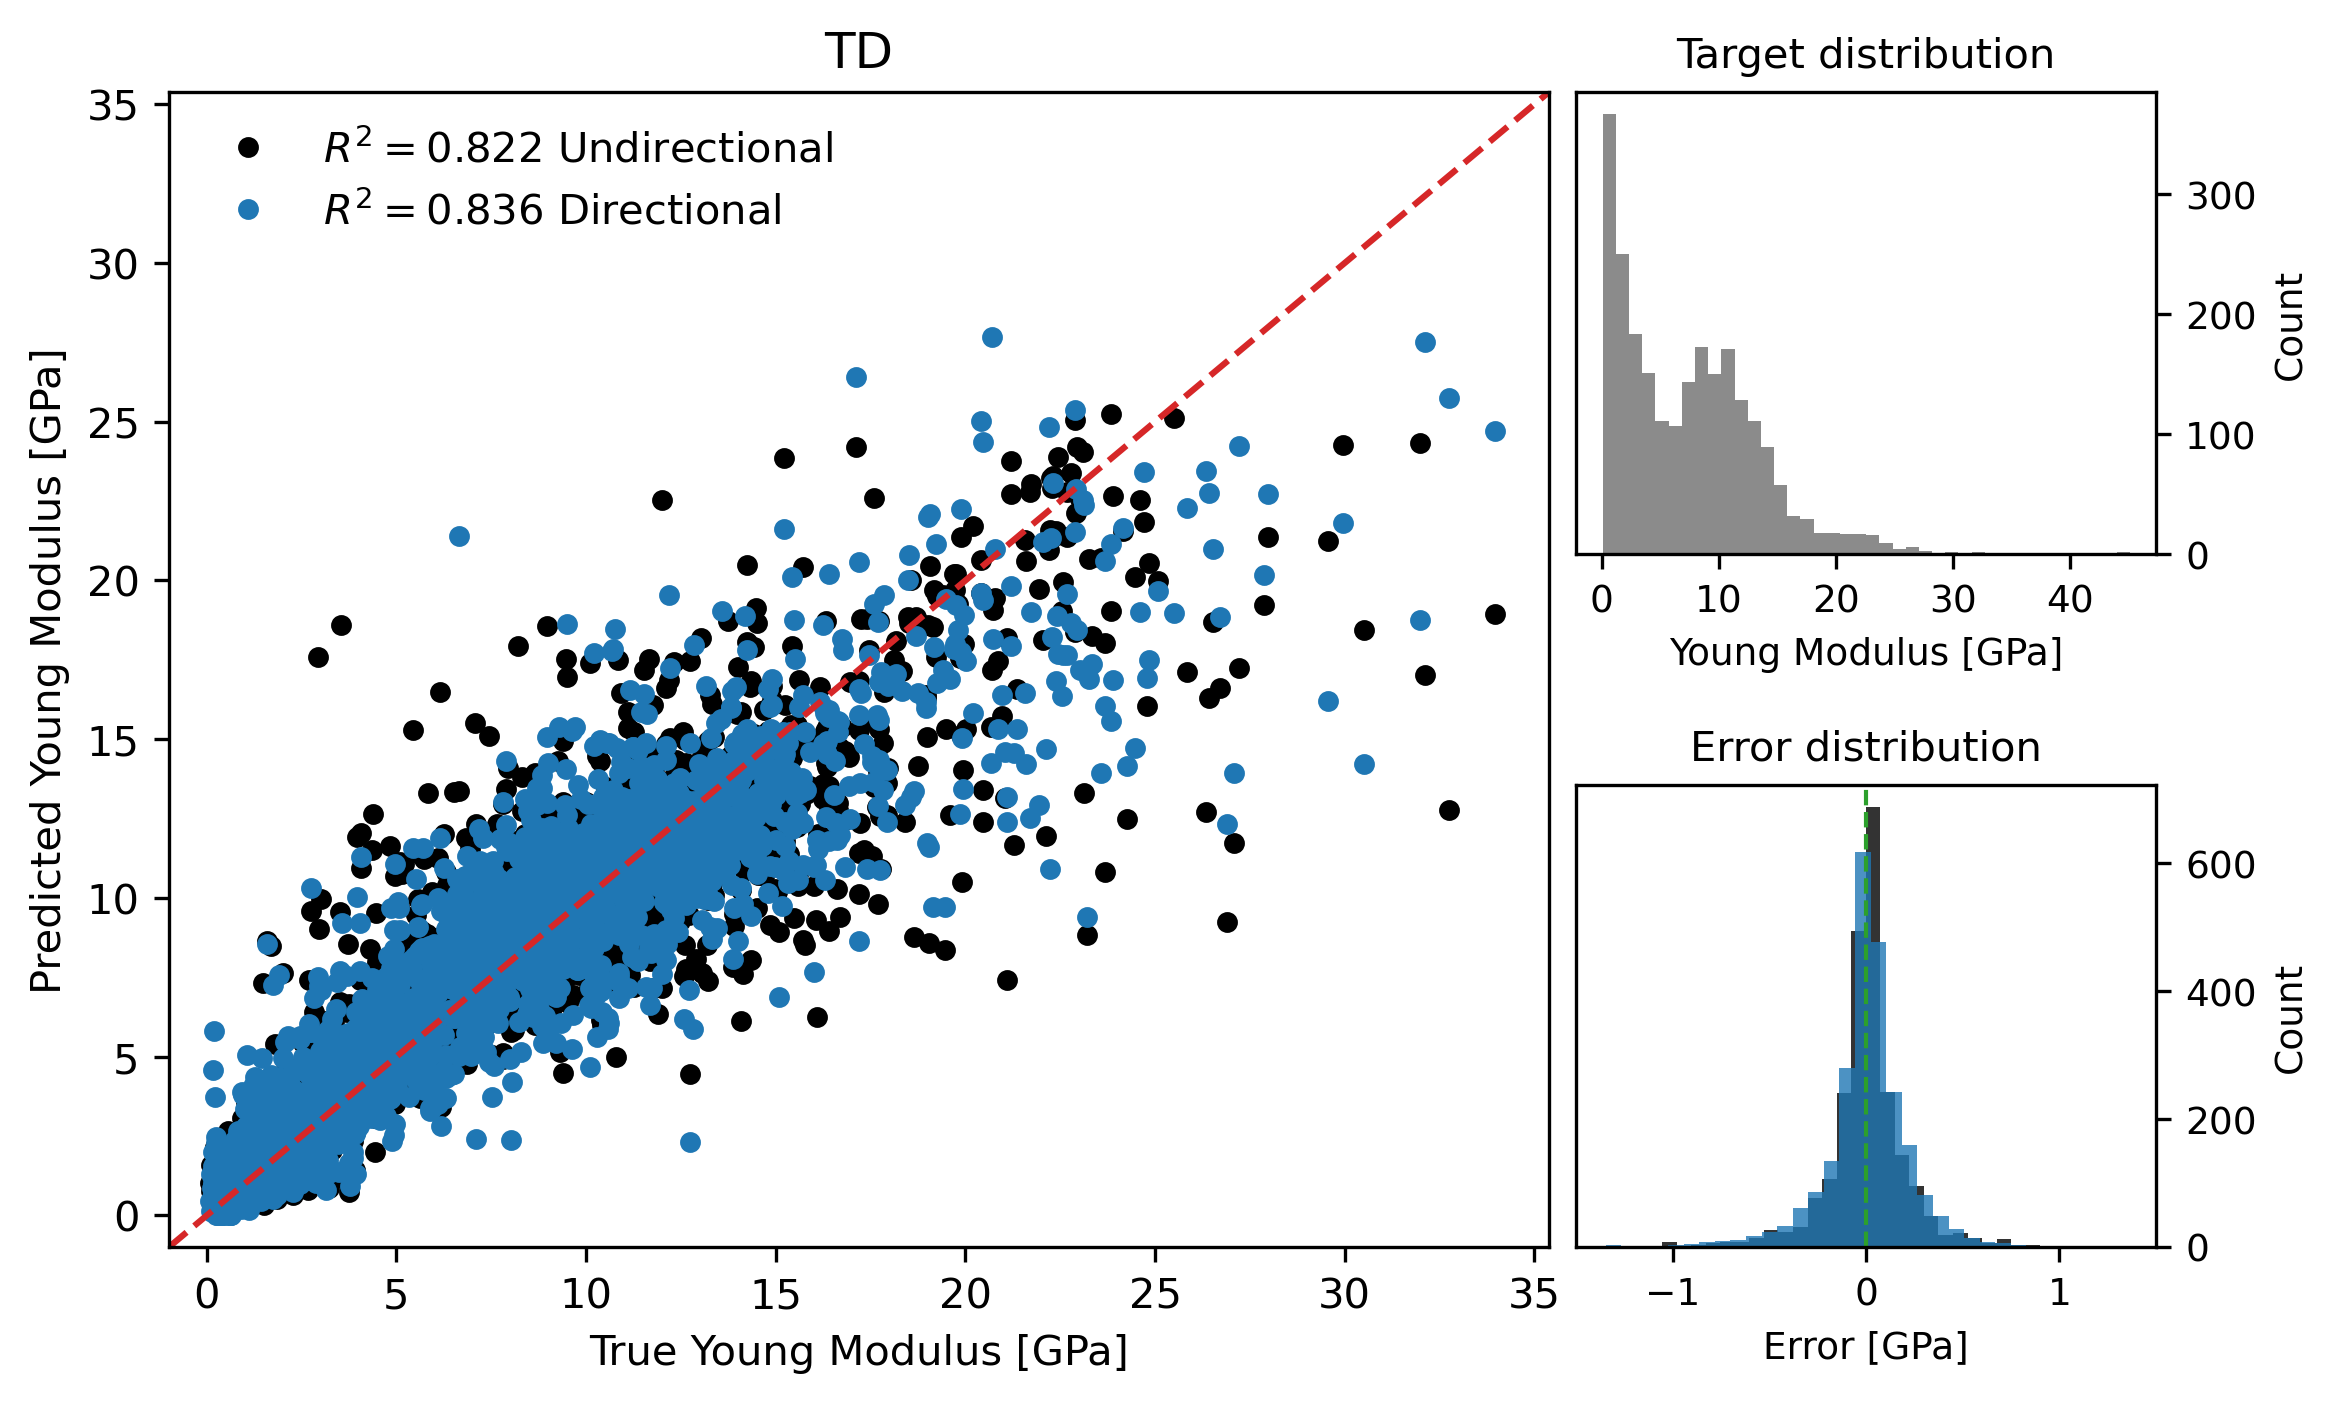
\includegraphics[width=0.495\linewidth]{scatter_td.png}
    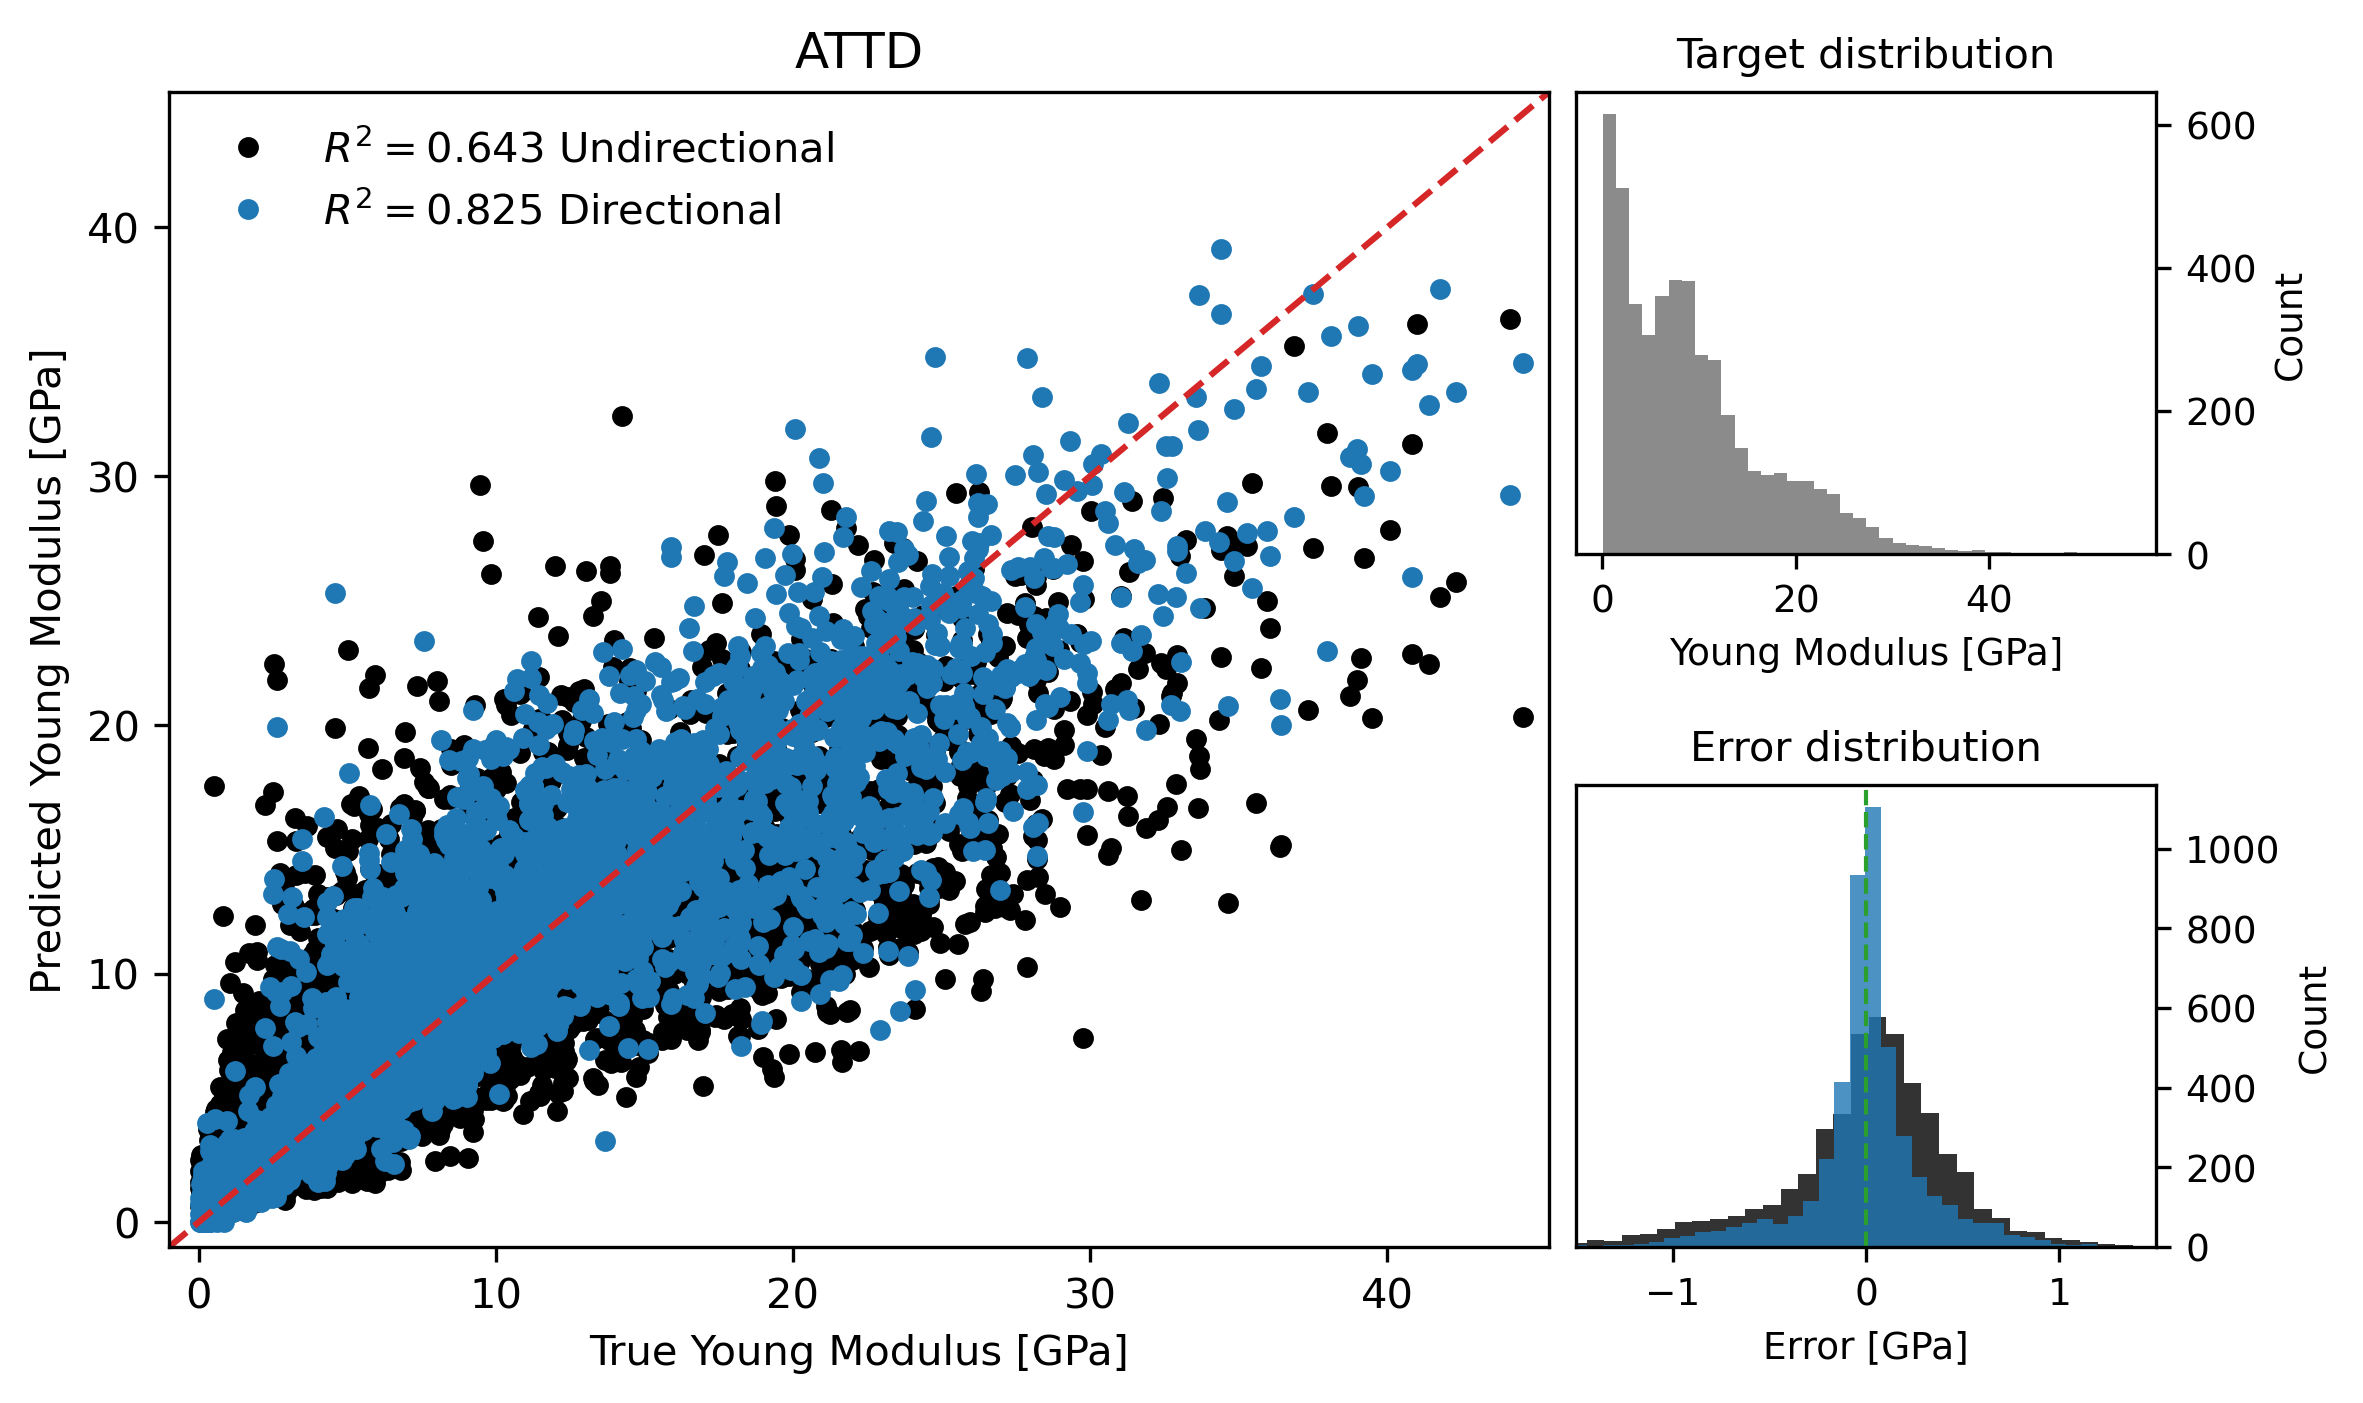
\includegraphics[width=0.495\linewidth]{scatter_attd.png}
    \caption{The same as Figure \ref{fig:scatter_rtp} but for TD dataset (left panel) and ATTD dataset (right panel).
    }
    \label{fig:scatter_td}
\end{figure}


To verify that the observed trends are not specific to the RTP model or to a
particular class of microstructures, additional datasets were considered.
Specifically, a Topologically Diverse (TD) dataset was constructed to include porous
microstructures spanning a broad range of topologies (see Section \ref{sec:td_structures} and Section S1 in the Supplementary Information), while remaining statistically isotropic.
This dataset is characterized by low anisotropy, with
$\sigma(k)=0.14$ and $\sigma(L)=1.80$, and an average Young’s modulus of $7.46\,\mathrm{GPa}$.
For the TD dataset, the same qualitative trends observed for RTPxy persist.
ECP multifiltration descriptors outperform the PH descriptors in both directional and non-directional settings. 
Non-directional PH achieves only $R^2=0.596$ with MAE $=2.44\,\mathrm{GPa}$, whereas
non-directional ECP improves performance substantially to $R^2=0.815$ and MAE $=1.48\,\mathrm{GPa}$.
Directional descriptors again provide a consistent advantage in terms of $R^2$: directional
PH+ECP reaches $R^2=0.836$, outperforming all non-directional alternatives, while the latter have a slight advantage in terms of MAE for ECP and PH+ECP.
This reinforces the conclusion
that direction-aware topology is not detrimental even for nominally isotropic
datasets.

A limitation of the TD dataset is that anisotropy cannot be introduced in a controlled manner at the level of microstructure generation. To address this, an Anisotropic Transformed Topologically Diverse (ATTD) dataset was constructed by elongating the original structures along a single axis, thereby introducing moderate but systematic anisotropy. This procedure increases the spectral anisotropy variability to $\sigma(k)=0.20$, while the correlation-length-based variability becomes $\sigma(L)=1.74$, and the average Young’s modulus increases to $9.36\,\mathrm{GPa}$.
Although ATTD is more anisotropic than TD—as reflected by the larger value of $\sigma(k)$—the value of $\sigma(L)$ is slightly lower. This stems from the definition of the correlation-length measure, which depends on the integral of the autocorrelation function up to its first zero crossing. In the TD and ATTD datasets, where structures are not generated from spectrally controlled random fields, the autocorrelation does not necessarily decay monotonically, and the elongation procedure can reduce variability in the position of the first zero crossing across samples. As a result, the spread of $L$ values may decrease even when directional anisotropy increases. In this context, $L$ serves primarily as an auxiliary real-space measure complementing the more sensitive spectral indicator $k$.

For the ATTD dataset, the benefits of directional topology become
more pronounced. Directional ECP improves predictive performance from $R^2=0.653$ in the
non-directional case to $0.815$, while directional PH+ECP achieves the highest
accuracy with $R^2=0.825$ and the lowest MAE of $2.06\,\mathrm{GPa}$.
In contrast, non-directional PH+ECP remains comparatively weak
($R^2=0.643$, MAE $=3.33\,\mathrm{GPa}$).
These results closely mirror those observed for RTPxz, demonstrating that the
relationship between anisotropy and the effectiveness of directional
descriptors is not restricted to RTP microstructures, but extends to a broader
class of porous topologies.

Figure~\ref{fig:scatter_td} compares predicted and FFTMAD-computed Young’s modulus for the TD (left) and ATTD (right) datasets. For the isotropic TD dataset, directional and non-directional topological descriptors yield comparable accuracy, with predictions clustered near perfect agreement. Introducing moderate anisotropy in ATTD leads to a clear separation: directional descriptors preserve tight alignment with the diagonal, while non-directional descriptors show increased scatter. As in the RTP datasets (Figure~\ref{fig:scatter_rtp}), this highlights that directional topology becomes increasingly informative as anisotropy strengthens, even for structurally diverse porous systems.


Across the TD and ATTD datasets, convolutional neural networks trained directly on voxelized structures achieve high accuracy, with $R^2 = 0.976$ for TD and $R^2 = 0.894$ for ATTD (Table~\ref{tab:metrics}). However, the performance gap between CNNs and topological models decreases as anisotropy increases and directional PH+ECP descriptors are used.
For the isotropic TD dataset ($\sigma(k)=0.14$), directional PH+ECP reaches $R^2 = 0.836$, yielding a gap of $0.140$ relative to the CNN. For the moderately anisotropic ATTD dataset ($\sigma(k)=0.20$), this gap reduces to $0.069$ ($R^2 = 0.825$ vs.\ $0.894$). A similar trend appears in the RTP datasets: the gap is $0.041$ for RTPxy and only $0.006$ for the strongly anisotropic RTPxz case, where directional PH+ECP nearly matches the CNN baseline ($R^2 = 0.978$ vs.\ $0.985$).
These results indicate that the CNN advantage largely reflects its ability to capture anisotropic structural information, which directional topological descriptors encode explicitly and increasingly effectively as anisotropy strengthens.


Taken together, the results across all datasets lead to several general
conclusions.
First, multifiltration ECP descriptors consistently outperform PH when used
alone, regardless of dataset or anisotropy level.
Second, combining PH and ECP yields the most accurate and stable topological
representations across all considered regimes.
Third, directional descriptors uniformly dominate non-directional ones for non-isotropic datasets and have virtually identical performance for isotropic datasets, leaving little practical justification for
the latter.
Finally, the advantage of directional topology increases systematically with
structural anisotropy, a trend observed consistently for both RTP and non-RTP
microstructures.
These findings highlight the robustness and generality of topological data
analysis as a framework for linking complex porous microstructures to
mechanical response, and underscore its potential as an interpretable,
low-dimensional alternative to purely voxel-based learning approaches.


\section{Summary}
\label{sec:summary}

Direction-dependent properties in porous materials pose a structural learning problem in which symmetry breaking with respect to the loading axis is essential. This work demonstrates that incorporating directional information into topological data analysis provides a significant advantage for predicting direction-dependent elastic properties of porous structures. Standard topological descriptors, while effective at capturing multiscale connectivity and void structure, are inherently isotropic and therefore insufficient for modeling anisotropic mechanical response. By embedding the loading direction directly into the filtration functions used for persistent homology and Euler characteristic profiles, the proposed direction-aware construction lifts this intrinsic isotropy and encodes mechanically relevant anisotropic topology in a compact representation.

Across multiple datasets spanning weak to strong anisotropy, direction-aware persistent homology and Euler characteristic profiles systematically improve predictive performance for uniaxial Young’s modulus compared with direction-agnostic topology, with gains that grow as structural anisotropy strengthens. The effect is most pronounced for strongly anisotropic structures (RTPxz), where direction-aware topology yields large improvements in both explained variance ($R^2$) and mean absolute error (MAE), reducing prediction errors by several-fold and nearly matching a voxel-based CNN baseline. For nominally isotropic ensembles (RTPxy and TD), directional descriptors remain uniformly competitive and typically increase $R^2$ (while occasionally inducing minor changes in MAE), indicating that direction-aware topology captures subtle mechanically relevant organization even when macroscopic anisotropy is weak.

Among descriptor families, multifiltration Euler characteristic profiles (ECP) consistently provide stronger predictive signal than persistent homology (PH) when used alone, and their combination (PH+ECP) produces the most accurate and stable models across all considered regimes. Moreover, as anisotropy increases (RTPxz and ATTD), the performance gap between topological models and convolutional neural networks trained directly on voxelized structures narrows substantially, demonstrating that a significant portion of the predictive power of high-dimensional image-based models can be recovered through compact, physics-informed, direction-aware topological summaries.

From the perspective of porous-materials modeling, these results establish a general, geometry-agnostic route for encoding anisotropic connectivity and alignment effects—key determinants of stiffness—without relying on handcrafted geometric descriptors or expensive end-to-end training on voxel grids. More broadly, the proposed direction-aware TDA framework provides a transferable and low-dimensional alternative (or complement) to voxel-based deep learning for structure–property prediction in porous media, with natural extensions to other direction-dependent properties such as yield strength, elastic tensors, permeability, and transport coefficients governed by anisotropic microstructural organization.

\subsection*{Code and Data Availability}
A complete implementation of all methods used in this study is available in the accompanying GitHub repository at \url{https://github.com/dioscuri-tda/direction-aware-tda-for-porous-materials}. The repository includes the full codebase for computing directional and non-directional topological descriptors, training the CatBoost and CNN models, reproducing all numerical experiments, and generating the figures reported in the manuscript. It also contains all datasets used in this work, including voxelized porous structures stored as \texttt{.npy} files, FFTMAD-computed Young’s modulus values, and vectorized PH, ECP, and PH+ECP descriptors. Ready-to-use databases, training scripts, and detailed instructions for reproducing every result are provided to ensure full transparency and straightforward replication of the presented findings.

\subsection*{Funding}
Financial support from the PORMETALOMICS project, funded by the Spanish
Ministry for Science, Innovation, and Universities (award no.
PCI2022-132975) and the National Science Centre, Poland (project no.
2021/03/Y/ST5/00232) within the M-ERA.NET 3 call, is gratefully acknowledged. 
This project has received funding from the European Union’s Horizon 2020 research and innovation programme under grant agreement No 958174.

This research is financed under Dioscuri, a programme initiated by the
Max Planck Society, jointly managed with the National Science Centre
in Poland, and mutually funded by Polish Ministry of Science and
Higher Education and German Federal Ministry of Research,
Technology and Space.

\section*{Declarations}
\subsection*{Author Contributions Statement}
R.T., M.B., and J.M. wrote the main manuscript. R.T., M.B., and B.N. generated the microstructures. R.T. and M.B. performed the FFTMAD simulations. R.T. developed the machine-learning code and ran computations. M.B., J.M., and P.D. designed and implemented the topological data analysis framework and reviewed the machine-learning and FFTMAD workflows. R.T., M.B., J.M., B.N., and P.D. contributed to the methodology. P.D., M.H., and B.N. provided computational resources. P.D. and M.H. supervised project administration. R.T. prepared all figures except Figure 3, which J.M. and M.B prepared. All authors contributed to formal analysis, validation of the results, and reviewed the final version of the manuscript. 

\subsection*{Competing Interests}
The authors declare no competing interests.

\clearpage

% Supplement-style numbering
\setcounter{section}{0}
\setcounter{figure}{0}
\setcounter{table}{0}
\setcounter{equation}{0}

\renewcommand{\thesection}{S\arabic{section}}
\renewcommand{\thesubsection}{S\arabic{section}.\arabic{subsection}}
\renewcommand{\thesubsubsection}{S\arabic{section}.\arabic{subsection}.\arabic{subsubsection}}
\renewcommand{\thefigure}{S\arabic{figure}}
\renewcommand{\thetable}{S\arabic{table}}
\renewcommand{\theequation}{S\arabic{equation}}
\begin{center}
\Huge{Supplementary Information}
\vspace{5cm}
\end{center}

\section{Topologically Diverse (TD) Dataset}
The RTP dataset is described in detail in the main text. All porous structures used in this study—including the RTP, TD, and ATTD datasets—are openly available in the dedicated repository associated with this paper: \url{https://github.com/dioscuri-tda/direction-aware-tda-for-porous-materials}. 
The repository also provides a utility for converting the voxelized data into VTK format, enabling straightforward visualization and rendering using standard tools such as ParaView.

\subsection{Generation of porous structures}
\subsubsection{Random Voronoi structures}\label{app:voronois}

600 random Voronoi structures were generated. For each structure, between 3 and 12 points were sampled from a unit cell (randomly, uniform distribution), with the space between them tesselated into Voronoi regions and the edges between regions used as a skeleton for the structure. The voxels traversed by the edges are approximated using the Bresenham's Line Algorithm~\cite{bresenham1965algorithm} and included within the structure. The edges are thickened to form struts with a square-shaped cross-section, with the side length of the square randomly drawn from the uniform distribution between 0.06 and 0.14. In order to guarantee periodicity of the structure, copies of the original points are generated in cells neighbouring the unit cell as well and the Voronoi tesselation of space, voxelisation of edges and subsequent thickening is conducted within the neighbouring cells as well (see Fig. \ref{fig:voronoi} for a visualization of a 2D version of the procedure), with the neighboring cells discarded at the last stage of the procedure. 

\begin{figure}[h!]
    \centering
    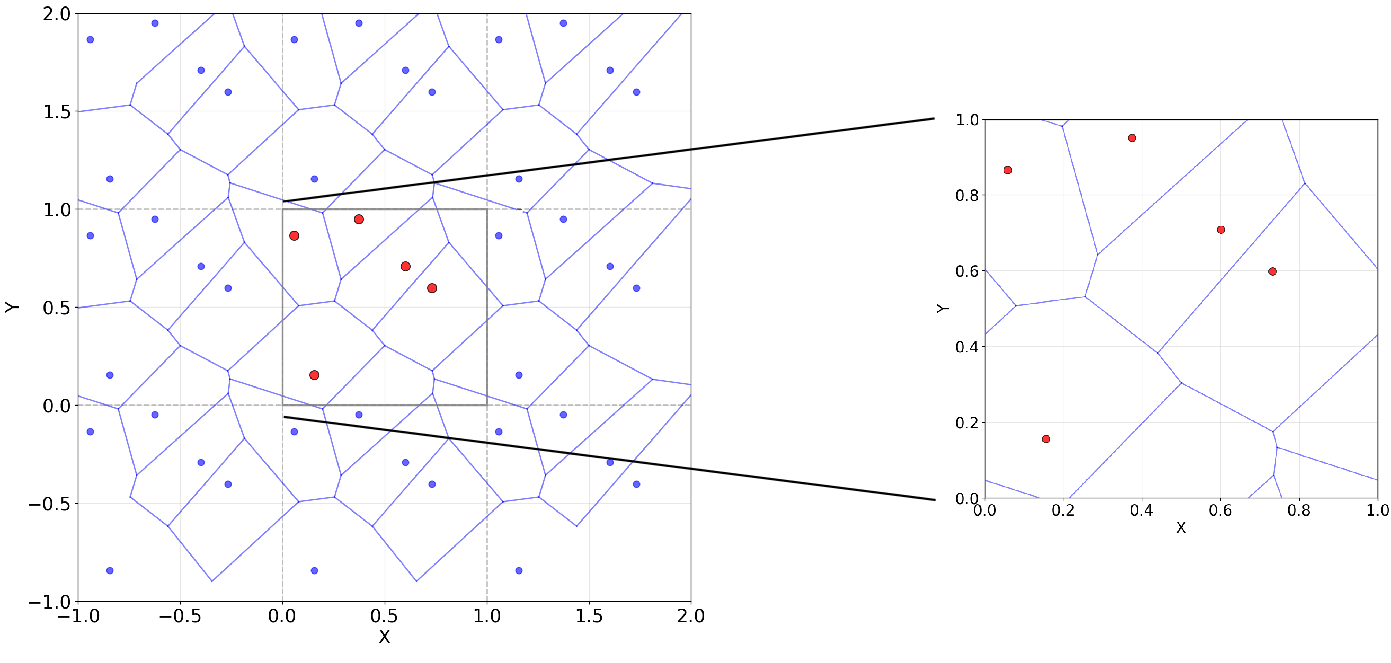
\includegraphics[width=0.89\linewidth]{Voronoi.png}
    \caption{A 2D visualisation of the algorithm for generating random Voronoi structures satisfying periodic boundary conditions.}
    \label{fig:voronoi}
\end{figure}

\subsubsection{Zeolites}\label{sec:zeolites}

More than 3000 predicted zeolitic structures were recovered from Michael Deem's database~\cite{C0CP02255A, deem2023pcod}. Each structure is described by the basis cell vector and the locations of Si and O atoms in a unit cell. We restricted the studies to structures with a perpendicular shape of the unit cell, which still left over 1500 structures. We transformed the structures from perpendicular to the normalized $1\times1\times1$ cubic volume by stretching/compression. We thickened the edges by dilation to form struts with a square-shaped cross-section of side length 0.12. We used 300 randomly drawn structures from the dataset and connected the locations of the Si atoms in these structures after the stretching/compression to the locations of their nearest Si neighbors (O atoms were not used in the structure). The connections formed the skeleton of the structure. Periodic boundary conditions were guaranteed by a procedure similar to the one used for random Voronoi structures, involving generating copies of the original Si atom locations in cells neighbouring the unit cell and connecting them to their nearest neighbours as well. Another 299 structures were created on the basis of different randomly drawn structures from using Michael Deem's database~\cite{C0CP02255A, deem2023pcod} using the same algorithm, but with using 0.04 instead of 0.12 as the side length of the square-shaped cross-section of the struts.  
This gives a total of 580 zeolite structures.  %599

\subsubsection{Diamond structures}

299 diamond-resembling structures were generated. Each structure was generated by creating within the unit cell 8 vertices corresponding to atoms in a diamond lattice and creating between the vertices edges corresponding to bonds between the atoms. The precise locations of the vertices were determined by adding a stochastic displacement to the location of the corresponding atom in the diamond lattice. Each of the three-dimensional components of the stochastic displacement for all vertices in a given lattice were drawn from a normal distribution with a standard deviation $\epsilon$ itself drawn from a uniform distribution between 0 and 0.1 (compare to 1.0 being the length of the side of a unit cell). That way, the amount of stochasticity was varied between the structures. The edges connecting the vertices were thickened via dilation to form struts with square-shaped cross-sections, with the length of the side of the cross-section drawn from a uniform distribution between 0.06 and 0.26. That way, the volume fraction was varied between structures.

\subsubsection{Cubic structures}

300 structures resembling a simple cubic strut were generated using the procedure used for diamond structures, with the only difference the 8 initiating points are not the locations of atoms in a diamond structures like in the former dataset, but instead the following set of points: [0, 0, 0],
        [0.5, 0, 0],
        [0, 0.5, 0],
        [0, 0, 0.5],
        [0, 0.5, 0.5],
        [0.5, 0, 0.5],
        [0.5, 0.5, 0],
        [0.5, 0.5, 0.5]. Replicating further steps from the procedure used to generate the diamond-like structures leads to structures resembling a classical cubic strut, with varying thicknesses of the struts and levels of randomization in locations of the struts' vertices. 


\subsubsection{Splines}

To generate a family of smooth porous morphologies, we construct a random \emph{periodic} scalar field on the unit cell and then threshold it.
Let $n=\texttt{sampling}$ be the number of spline control points per direction and draw i.i.d.\ coefficients
\begin{equation}
r_{ijk}\sim\mathcal U(0,1),\qquad i,j,k=1,\dots,n .
\end{equation}
In \textsc{Mathematica}, the command
\texttt{BSplineFunction} builds a trivariate tensor-product B-spline field
(with \texttt{SplineDegree->3}, \texttt{SplineClosed->True}, \texttt{SplineKnots->"Unclamped"}), i.e.
\begin{equation}
f(x,y,z)=\sum_{i=1}^{n}\sum_{j=1}^{n}\sum_{k=1}^{n}
r_{ijk}\,N_{i,3}(x)\,N_{j,3}(y)\,N_{k,3}(z),
\label{eq:spline_field}
\end{equation}
where $\{N_{i,3}\}$ are cubic B-spline basis functions (defined via the Cox--de Boor recursion), and the ``closed'' setting enforces periodicity across the cell boundaries \cite{deBoor1978,wolframBSplineFunction}.

A binary structure is then obtained as a super-level set. Using wrapped (periodic) coordinates
$\tilde{\boldsymbol{x}}=(x\bmod 1,\,y\bmod 1,\,z\bmod 1)$ (implemented with \texttt{Mod}), we voxelize on an $L\times L\times L$ grid (here $L=80$) by
\begin{equation}
T_{abc}(t)=\mathbf{1}\Bigl\{\,f\!\bigl(\tfrac{a}{L},\tfrac{b}{L},\tfrac{c}{L}\bigr)\ge t\,\Bigr\},
\qquad a,b,c=0,\dots,L-1,
\label{eq:thresholding}
\end{equation}
and report the volume fraction
\begin{equation}
\phi(t)=\frac{1}{L^{3}}\sum_{a,b,c} T_{abc}(t).
\end{equation}
Varying the threshold $t$ (in our implementation, on an approximately uniform grid in $[0.35,0.50]$) produces two independent subsets of spline-based structures each, spanning a range of $\phi(t)$ while preserving smoothness and periodic tiling of the unit cell.
Total of 596 spline structures were used in the dataset.

\section{Results for RTPxyz dataset}
\begin{figure}
    \centering
    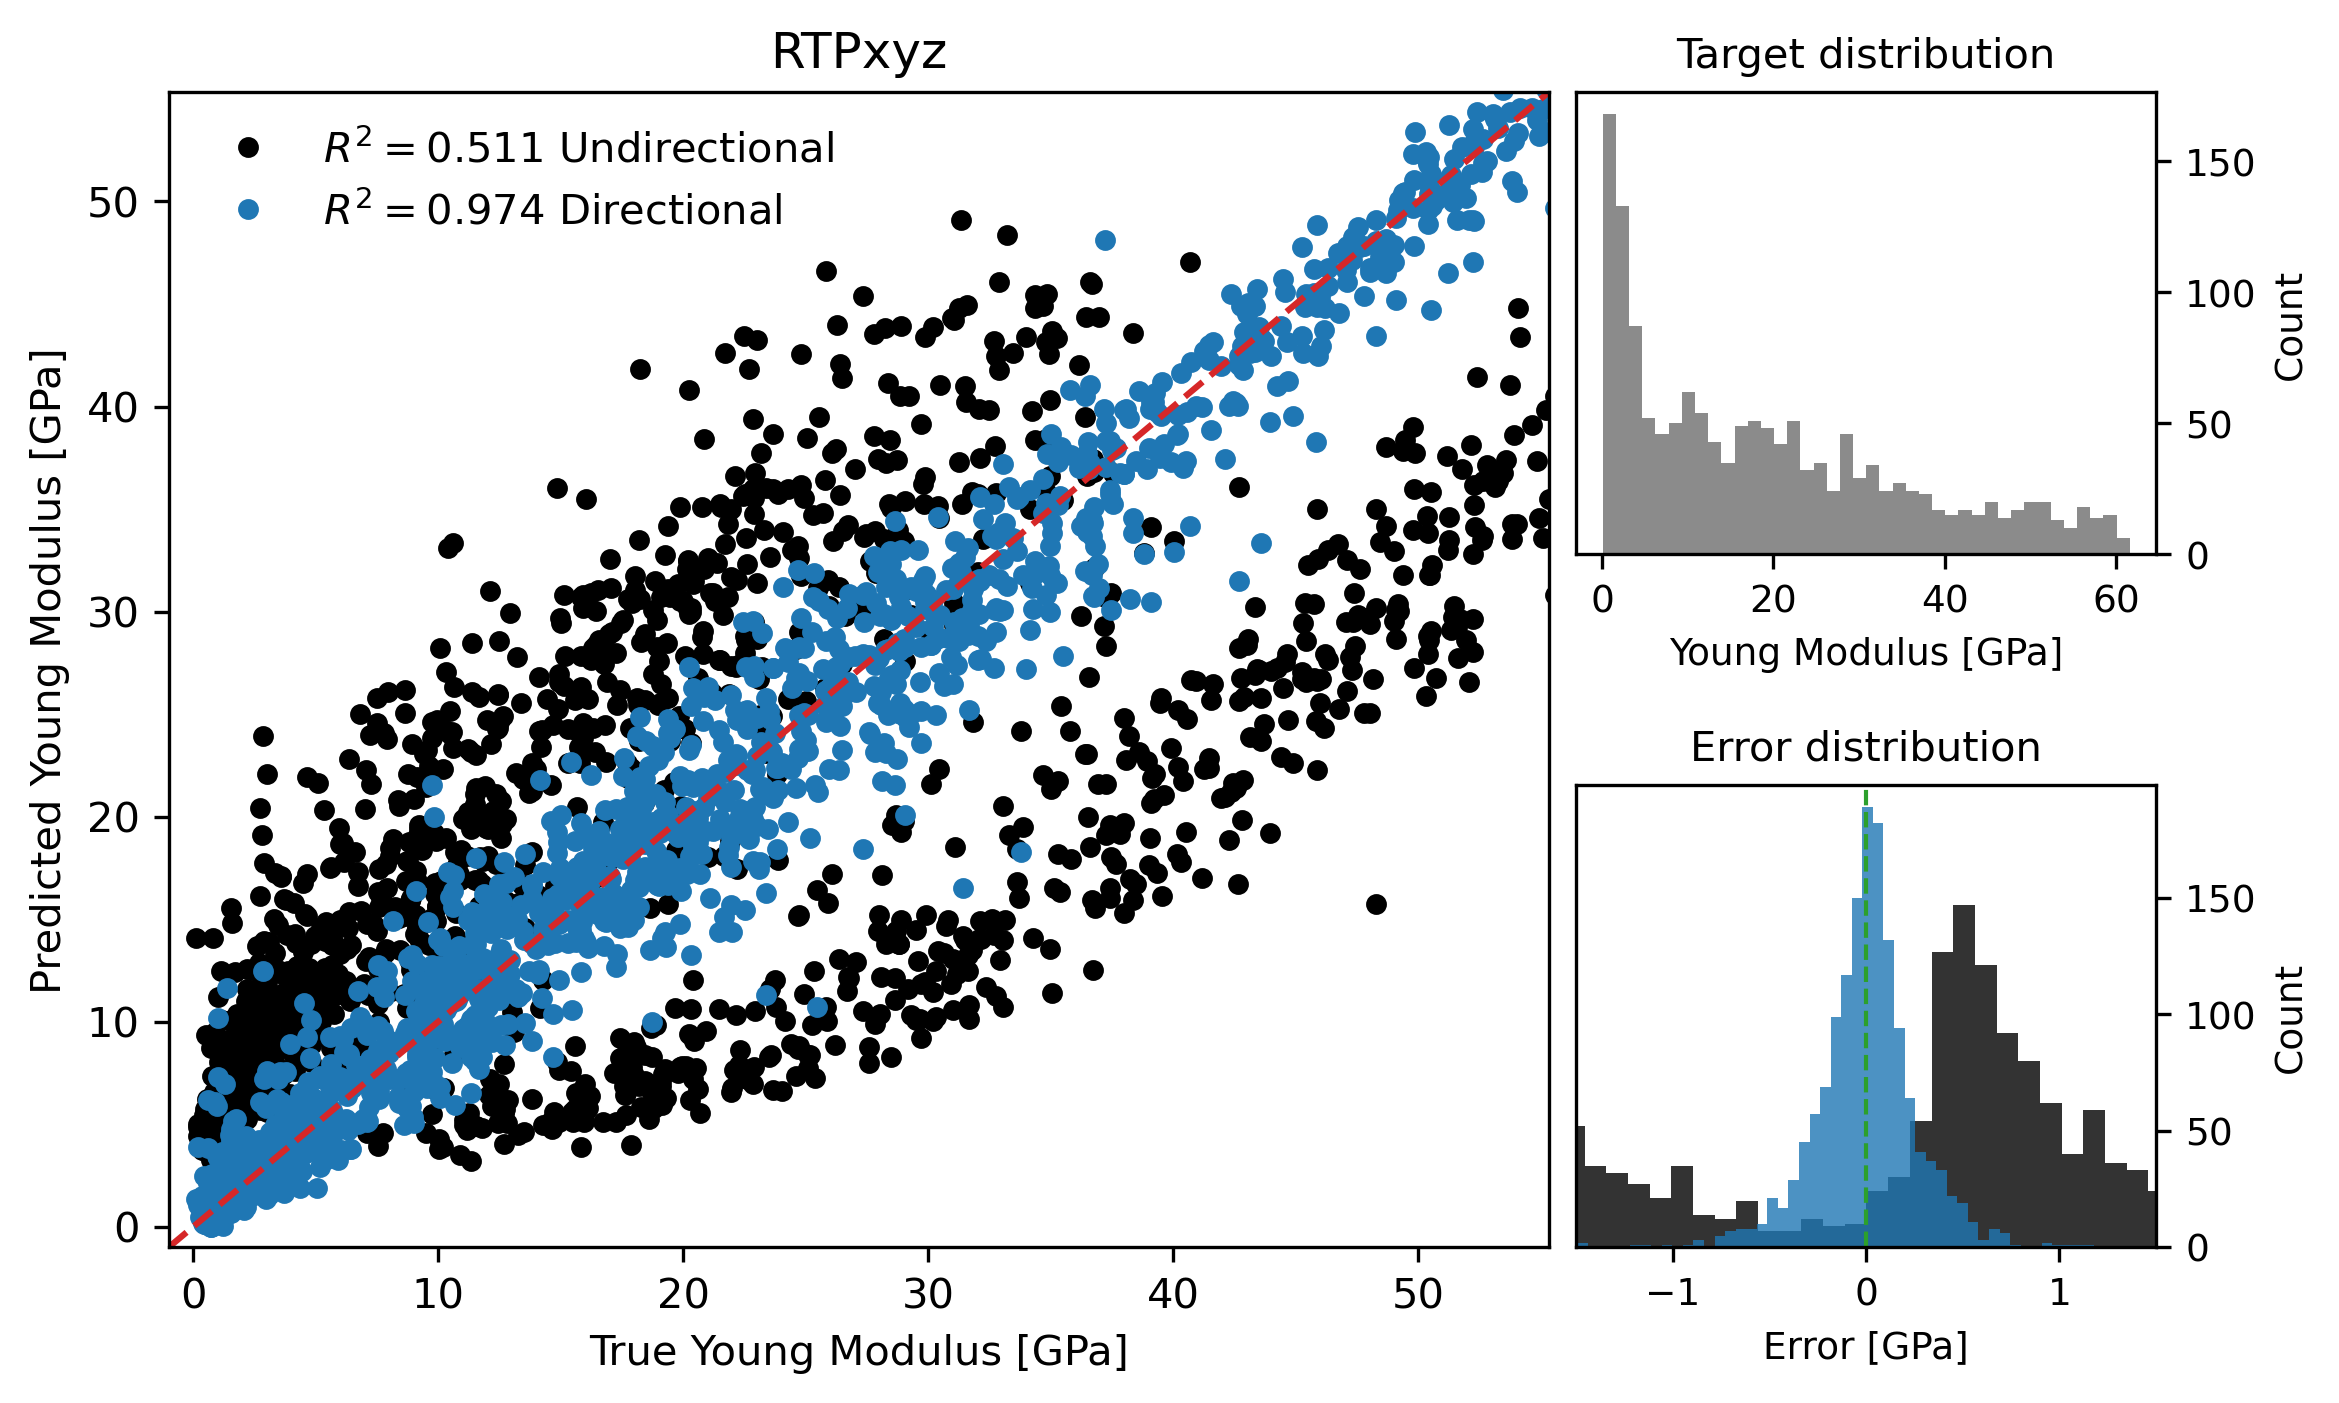
\includegraphics[width=0.75\textwidth]{scatter_rtp_xyz.png}
    \caption{Predicted versus FFTMAD-computed Young’s modulus for the RTPxyz dataset. The same as Figure 4 in the Manuscript but for the RTPxyz dataset. }
    \label{fig:scatter_rtp_xyz}
\end{figure} 

Models were additionally trained on the RTPxyz dataset, which aggregates Young’s modulus values computed for the RTP structures along all three Cartesian directions. This dataset comprises a total of 1500 samples, of which two thirds correspond to the mechanically easy axes ($x$ and $y$) and one third to the mechanically hard axis ($z$). The scatter plot of predicted versus FFTMAD-computed Young’s modulus for models trained with directional and non-directional descriptors is shown in Fig.~\ref{fig:scatter_rtp_xyz}, while the corresponding regression metrics are summarized in Table~\ref{tab:metrics_rtp_xyz}.

Models based on directional descriptors maintain high predictive accuracy, with predictions tightly clustered around the diagonal and a coefficient of determination of $R^2 = 0.974$. In contrast, models relying on non-directional descriptors perform poorly, achieving only $R^2 = 0.511$. The corresponding scatter plot reveals a pronounced bifurcation: predictions obtained from non-directional descriptors split into two distinct branches, one above and one below the diagonal.

\begin{table}[]
\centering
\caption{Cross-validated regression metrics for Young’s modulus prediction using CatBoost with PH, ECP, and PH+ECP topological summaries, and a CNN baseline trained directly on voxelized structures. Reported as average over 8 folds. The same as Table~1 in the manuscript but for the RTPxyz dataset.}
\label{tab:metrics_rtp_xyz}
\begin{tabular}{lcc|cc||l|rrrr}
\hline 
 & \multicolumn{2}{l}{} & \multicolumn{2}{|l||}{CNN baseline} &  & \multicolumn{2}{l}{Non-directional} & \multicolumn{2}{l}{Directional} \\
Dataset & $\sigma(k)$ & $\sigma(L)$ & $R^2$ & MAE & Method & $R^2$ & MAE & $R^2$ & MAE \\ \hline
RTPxyz & 0.38 & 1.77 & 0.990 & 1.88 & PH     & 0.509 & 13.26 & 0.548 & 13.61 \\
 &  &  &  &                        & ECP    & 0.493 & 15.11 & 0.974 & 3.09 \\
 &  &  &  &                        & PH+ECP & 0.511 & 9.94  & 0.974 & 2.89 \\ \hline
\end{tabular}
\end{table}


The upper branch (systematic overestimation) predominantly contains data points corresponding to compression along the mechanically easy $x$ and $y$ axes, where the true Young’s modulus is relatively low. The lower branch (systematic underestimation) consists mainly of samples compressed along the mechanically hard $z$ axis, where the true Young’s modulus is significantly higher. This clear separation demonstrates that non-directional descriptors fail to encode the loading direction and therefore cannot distinguish between mechanically inequivalent orientations of the same structure.

Only a small fraction of predictions obtained with non-directional descriptors lie close to the line of perfect agreement, which is reflected in the broadened and multimodal error distribution shown in the inset histogram. In contrast, no such branching behavior is observed for directional descriptors: predictions remain symmetrically distributed around the diagonal, indicating that direction-aware topology provides a consistent and physically meaningful representation of anisotropic mechanical response.

\section{Per-Fold Cross-Validation Performance}
The implemented cross-validation procedure allows for a direct comparison of the models within each fold, as identical train/validation/test splits are used throughout. This provides substantially more detailed insight than the averaged results reported in Table 1 of the manuscript.

The per-fold results for the $R^2$ and MAE metrics are presented in Tables~\ref{tab:fold_r2} and~\ref{tab:fold_mae}, respectively. The column Gain indicates whether the use of directional descriptors improves the performance, i.e., increases $R^2$ or decreases MAE. The last two rows of each table report the mean and standard deviation across folds for each method.

We report results for the PH+ECP descriptor on the RTPxz and RTPxy datasets, as this combination constitutes the main result of the paper. As shown in the tables, the improvement obtained by incorporating directional descriptors is consistent across all folds and for both datasets: $R^2$ increases and MAE decreases in every single split, demonstrating that the performance gain is systematic rather than incidental. The only exception is the standard deviation of $R^2$ for RTPxy, which is slightly higher for the directional descriptors compared to the non-directional variant.

\begin{table}[]
\caption{$R^2$ scores obtained in each cross-validation fold for the RTPxz and RTPxy datasets using the PH+ECP descriptor. Results for the CNN model are provided for reference. The column \textit{Gain} indicates whether the inclusion of directional descriptors improves performance (i.e., increases $R^2$). The last two rows report the mean and standard deviation across folds.}
\label{tab:fold_r2}
\begin{tabular}{r|rrlr|rrlrr}
\hline
\multicolumn{1}{l|}{$R^2$} & \multicolumn{4}{c|}{RTPxz} & \multicolumn{4}{c}{RTPxy} & \multicolumn{1}{l}{} \\
\multicolumn{1}{l|}{} & \multicolumn{3}{c}{PH+ECP} & \multicolumn{1}{l|}{CNN} & \multicolumn{3}{c}{PH+ECP} & \multicolumn{1}{l}{CNN} & \multicolumn{1}{l}{} \\
\multicolumn{1}{l|}{fold} & \multicolumn{1}{l}{Directional} & \multicolumn{1}{l}{Non-directional} & Gain & \multicolumn{1}{l|}{---} & \multicolumn{1}{l}{Directional} & \multicolumn{1}{l}{Non-directional} & Gain & \multicolumn{1}{l}{--} &  \\ \hline
1 & 0.9706 & 0.7213 & Yes & 0.9689 & 0.9176 & 0.9012 & Yes & 0.9852 &  \\
2 & 0.9829 & 0.8088 & Yes & 0.9876 & 0.9777 & 0.9587 & Yes & 0.9751 &  \\
3 & 0.9814 & 0.7638 & Yes & 0.9923 & 0.9265 & 0.9179 & Yes & 0.9889 &  \\
4 & 0.9726 & 0.7582 & Yes & 0.9899 & 0.9132 & 0.9013 & Yes & 0.9823 &  \\
5 & 0.9795 & 0.7018 & Yes & 0.9889 & 0.9408 & 0.9162 & Yes & 0.9892 &  \\
6 & 0.9798 & 0.7473 & Yes & 0.9776 & 0.9525 & 0.9035 & Yes & 0.9732 &  \\
7 & 0.9764 & 0.7866 & Yes & 0.9828 & 0.9532 & 0.9130 & Yes & 0.9863 &  \\
8 & 0.9816 & 0.7464 & Yes & 0.9884 & 0.9233 & 0.9169 & Yes & 0.9541 &  \\ \hline
\multicolumn{1}{l|}{Mean} & 0.9781 & 0.7543 & Yes & 0.9846 & 0.9381 & 0.9161 & Yes & 0.9793 &  \\
\multicolumn{1}{l|}{Std} & 0.0045 & 0.0340 & Yes & 0.0078 & 0.0221 & 0.0186 & No & 0.0118 &  \\ \hline
\end{tabular}
\end{table}

\begin{table}[]
\caption{The same as Table \ref{tab:fold_r2} but for MAE.}
\label{tab:fold_mae}
\begin{tabular}{r|rrlr|rrlrr}
\hline
\multicolumn{1}{l|}{MAE} & \multicolumn{4}{c|}{RTPxz} & \multicolumn{4}{c}{RTPxy} & \multicolumn{1}{l}{} \\
\multicolumn{1}{l|}{} & \multicolumn{3}{c}{PH+ECP} & \multicolumn{1}{l|}{CNN} & \multicolumn{3}{c}{PH+ECP} & \multicolumn{1}{l}{CNN} & \multicolumn{1}{l}{} \\
\multicolumn{1}{l|}{fold} & \multicolumn{1}{l}{Directional} & \multicolumn{1}{l}{Non-directional} & Gain & \multicolumn{1}{l|}{---} & \multicolumn{1}{l}{Directional} & \multicolumn{1}{l}{Non-directional} & Gain & \multicolumn{1}{l}{--} &  \\ \hline
1 & 2.116 & 7.532 & Yes & 2.269 & 2.051 & 2.202 & Yes & 0.871 &  \\
2 & 1.572 & 6.511 & Yes & 1.504 & 1.120 & 1.493 & Yes & 1.225 &  \\
3 & 1.631 & 6.803 & Yes & 1.185 & 1.512 & 1.763 & Yes & 0.701 &  \\
4 & 1.965 & 6.757 & Yes & 1.203 & 1.674 & 1.735 & Yes & 0.792 &  \\
5 & 1.820 & 7.821 & Yes & 1.380 & 1.764 & 2.087 & Yes & 0.735 &  \\
6 & 1.891 & 7.331 & Yes & 2.062 & 1.656 & 2.213 & Yes & 1.243 &  \\
7 & 2.119 & 6.788 & Yes & 2.021 & 1.850 & 2.396 & Yes & 1.060 &  \\
8 & 1.730 & 6.878 & Yes & 1.336 & 1.906 & 1.989 & Yes & 1.520 &  \\ \hline
\multicolumn{1}{l|}{Mean} & 1.855 & 7.053 & Yes & 1.620 & 1.692 & 1.985 & Yes & 1.018 &  \\
\multicolumn{1}{l|}{Std} & 0.207 & 0.454 & Yes & 0.430 & 0.284 & 0.300 & Yes & 0.293 &  \\ \hline
\end{tabular}
\end{table}

% \bibliographystyle{sn-mathphys-num}
% \bibliography{references}





\clearpage

\bibliographystyle{sn-mathphys-num}
\bibliography{references}



\end{document}
